\section{Datasets and Benchmarks in Action Recognition}
\label{chap:datasets}

Using publicly available dataset for evaluating action recognition algorithms has two main benefits:
\begin{enumerate}
    \item Collecting, annotating and storing video datasets is a tedious task, since videos have a higher dimensionality than images and especially deep learning algorithms require large amounts of training data. Additionally, the beginning and end of a performed action has to be included in the action label, possibly along with the spatial position of the action in the scene. Therefore using already existing datasets saves time in the development of action recognition algorithms.
    \item More importantly: Using the same datasets in different approaches, along with standardized evaluation schemes, enables the comparison between them. This is the basis of evaluating the quality of action recognition approaches. 
\end{enumerate}

Given the importance of datasets in the computer vision community, a couple of reviews have been published \cite{ahad_action_2011}\cite{liu_benchmarking_2011}\cite{hassner_critical_2013}\cite{chaquet_survey_2013}.
The review of \textcite{ahad_action_2011} and \textcite{liu_benchmarking_2011} were published back in 2011 and provide only a brief overview of benchmarking datasets.
\textcite{hassner_critical_2013} also review available datasets briefly and promote a completely different approach to benchmarking action recognition approaches, namely \textit{Action Similarity Labelling}, which is further describes in this below in this section.
\textcite{chaquet_survey_2013} provide a very comprehensive and detailed review of human action video datasets, which was published in 2013.

Building on \cite{chaquet_survey_2013}, this section gives a brief review of the most commonly used datasets and focusses on the newest ones.
All datasets in this section are publicly available.
Additionally, a review of datasets containing Activites of Daily Living (ADL) is given.
These datasets could be used to design and train a real-world action recognition system, to be used in assisted living environments.

\textcite{chaquet_survey_2013} provide a fine-grained classification according to the type of actions present in the datasets, as illustrated in figure~\ref{fig:datasetssurvey_taxonomy}.
\begin{figure}[H]
    \centering
    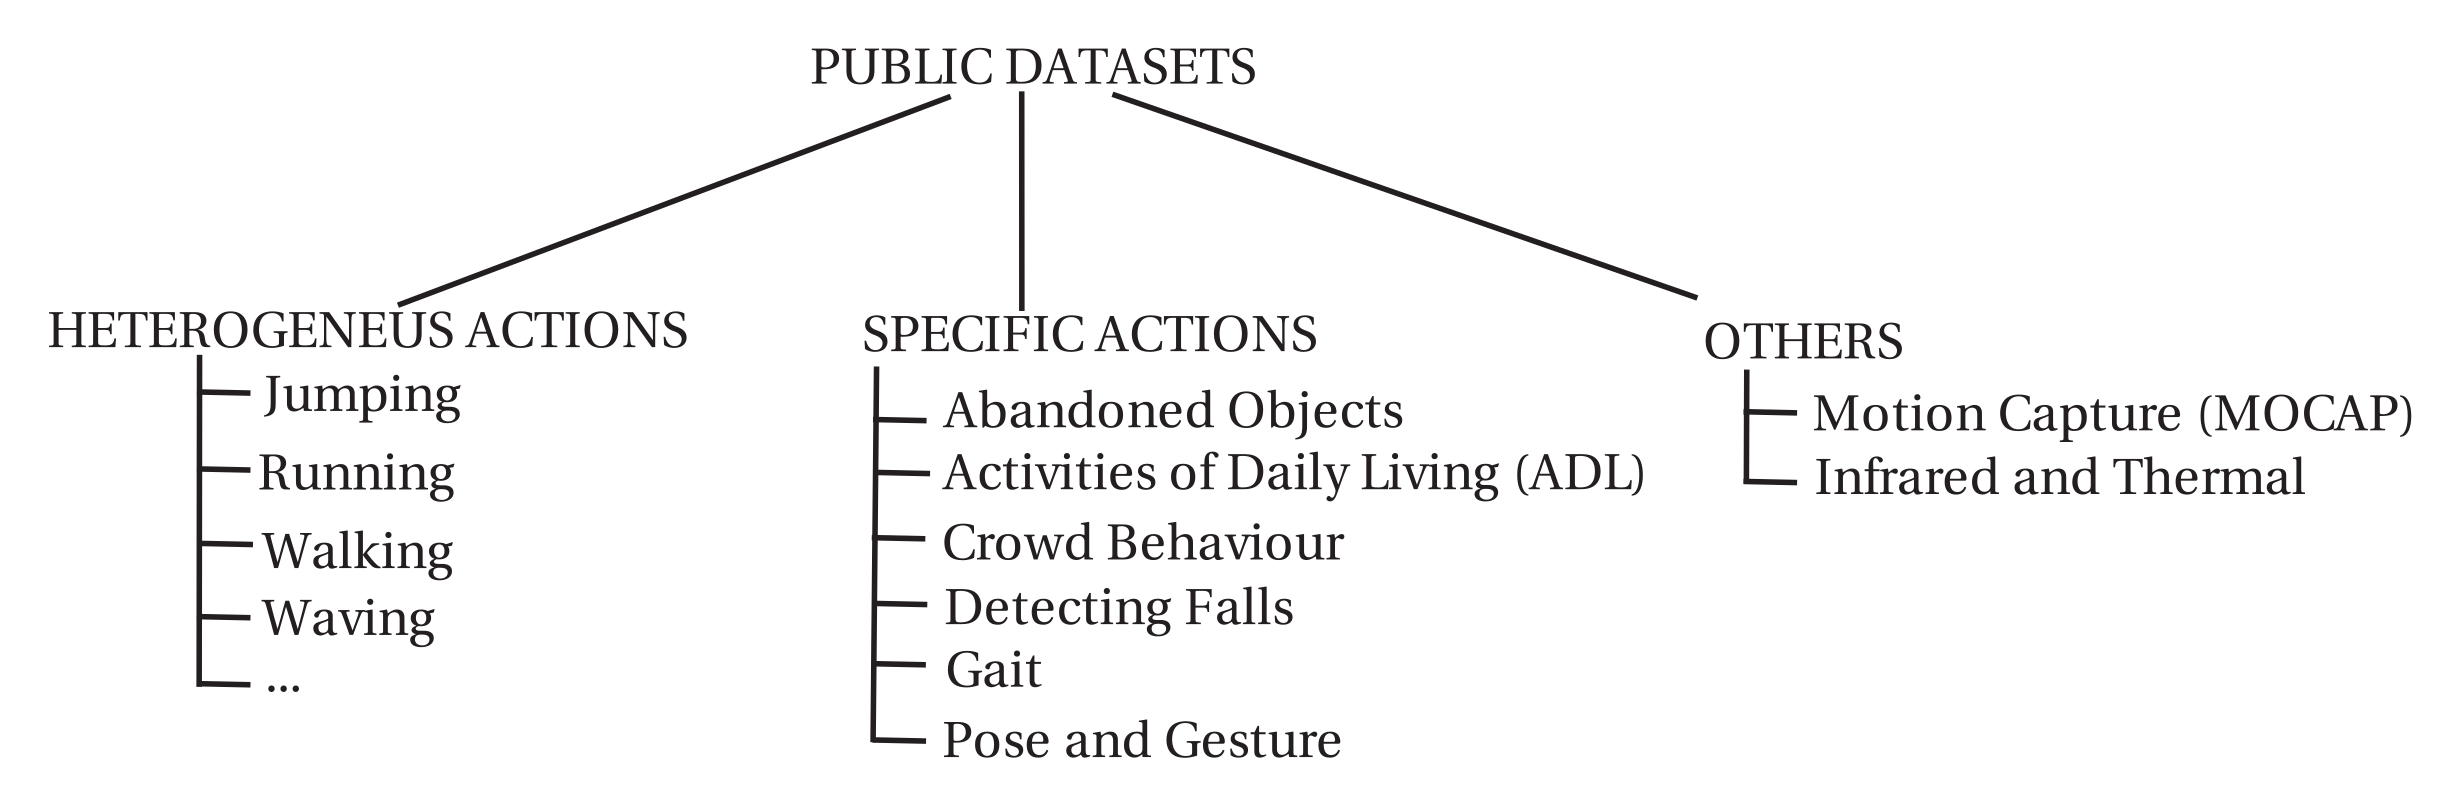
\includegraphics[width=\textwidth]{img_datasets/datasetssurvey_taxonomy}
    \caption{Taxonomy of publicly available datasets provided by \cite{chaquet_survey_2013}}
    \label{fig:datasetssurvey_taxonomy}
\end{figure}
\begin{description}
    \item[Heterogeneous Actions] describes the class of common actions that can appear in a wide variety of scenes and situations.
        Because of their generality, most benchmarking datasets, as well as the survey of \textcite{chaquet_survey_2013} focus on this kind of actions.
    \item[Specific Actions] denotes the class of action datasets that are used for training an action recognition system for a specific task such as fall detection, gait recognition or crowd behaviour recognition.
    \item[Others] denotes the category, that is specified by the technique used to capture the action datasets. Examples are Motion Capture, i.e.\ capturing human motion aided by special instruments such as joint markers and thermal or infrared imaging.
\end{description}

Since the actions of interest in this work are heterogeneous and can appear in any kind of context, we use a different classification scheme.
As proposed in \cite{hassner_critical_2013} action recognition datasets can be roughly categorized into three epochs, which differ in age, source of the videos and complexity.
\begin{enumerate}
    \item \textbf{Early Benchmarking Datasets} provide low resolution videos of a few basic action classes. These datasets are usually recorded under controlled conditions with static cameras, uncluttered backgrounds and actions are performed by actors.
    \item \textbf{Intermediate Benchmarking Datasets} are larger and more challenging for action recognition algorithms compared to early datasets. Actions in this class are usually sampled from television broadcasts or movies and provide uncontrolled conditions, moving cameras, cluttered backgrounds and occlusion. Given their source, videos in these datasets can be considered high-quality.
    \item \textbf{Modern Datasets} aim at providing a large number of action classes and examples. Videos in modern datasets are most often sampled from YouTube to provide real-world footage with varying resolutions, different lighting conditions, cuts, cluttered backgrounds and moving cameras. These are the most challennging datasets to date.
\end{enumerate}


\subsection{Early Benchmarking Datasets -- Controlled Conditions}

\subsubsection{KTH -- 2004}
%\cite{schuldt_recognizing_2004}\\
The KTH dataset \cite{schuldt_recognizing_2004} is an early and widely used benchmarking dataset containing grayscale video-clips of atomic actions performed by $25$ different actors in controlled environments.
The dataset was created and released by the swedish KTH Royal Institute of Technology in 2004.
It's considered a milestone in computer vision \cite{chaquet_survey_2013} and is the most commonly used publicly available dataset of human actions \cite{baccouche_sequential_2011}.
It was the largest video dataset of human actions at that time and enabled a systematic and comparable evaluation of action recognition algorithms by using the same input data.

Dataset details: \cite{schuldt_recognizing_2004}
\begin{itemize}
    \item $2391$ action instances in controlled conditions.
    \item $6$ action classes recorded in $4$ different scenarios (see figure \ref{fig:kth_example}).
    \item $25$ different actors.
    \item Homogeneous, uncluttered backgrounds.
    \item Static camera.
    \item $160 \times 120$ pixels video-resolution @ $25$\textit{fps}
    \item $4s$ average sequence length
\end{itemize}

Figure ~\ref{fig:kth_example} shows example frames of the KTH dataset, ordered by action class and recording scenarios.

\begin{figure}[H]
    \centering
    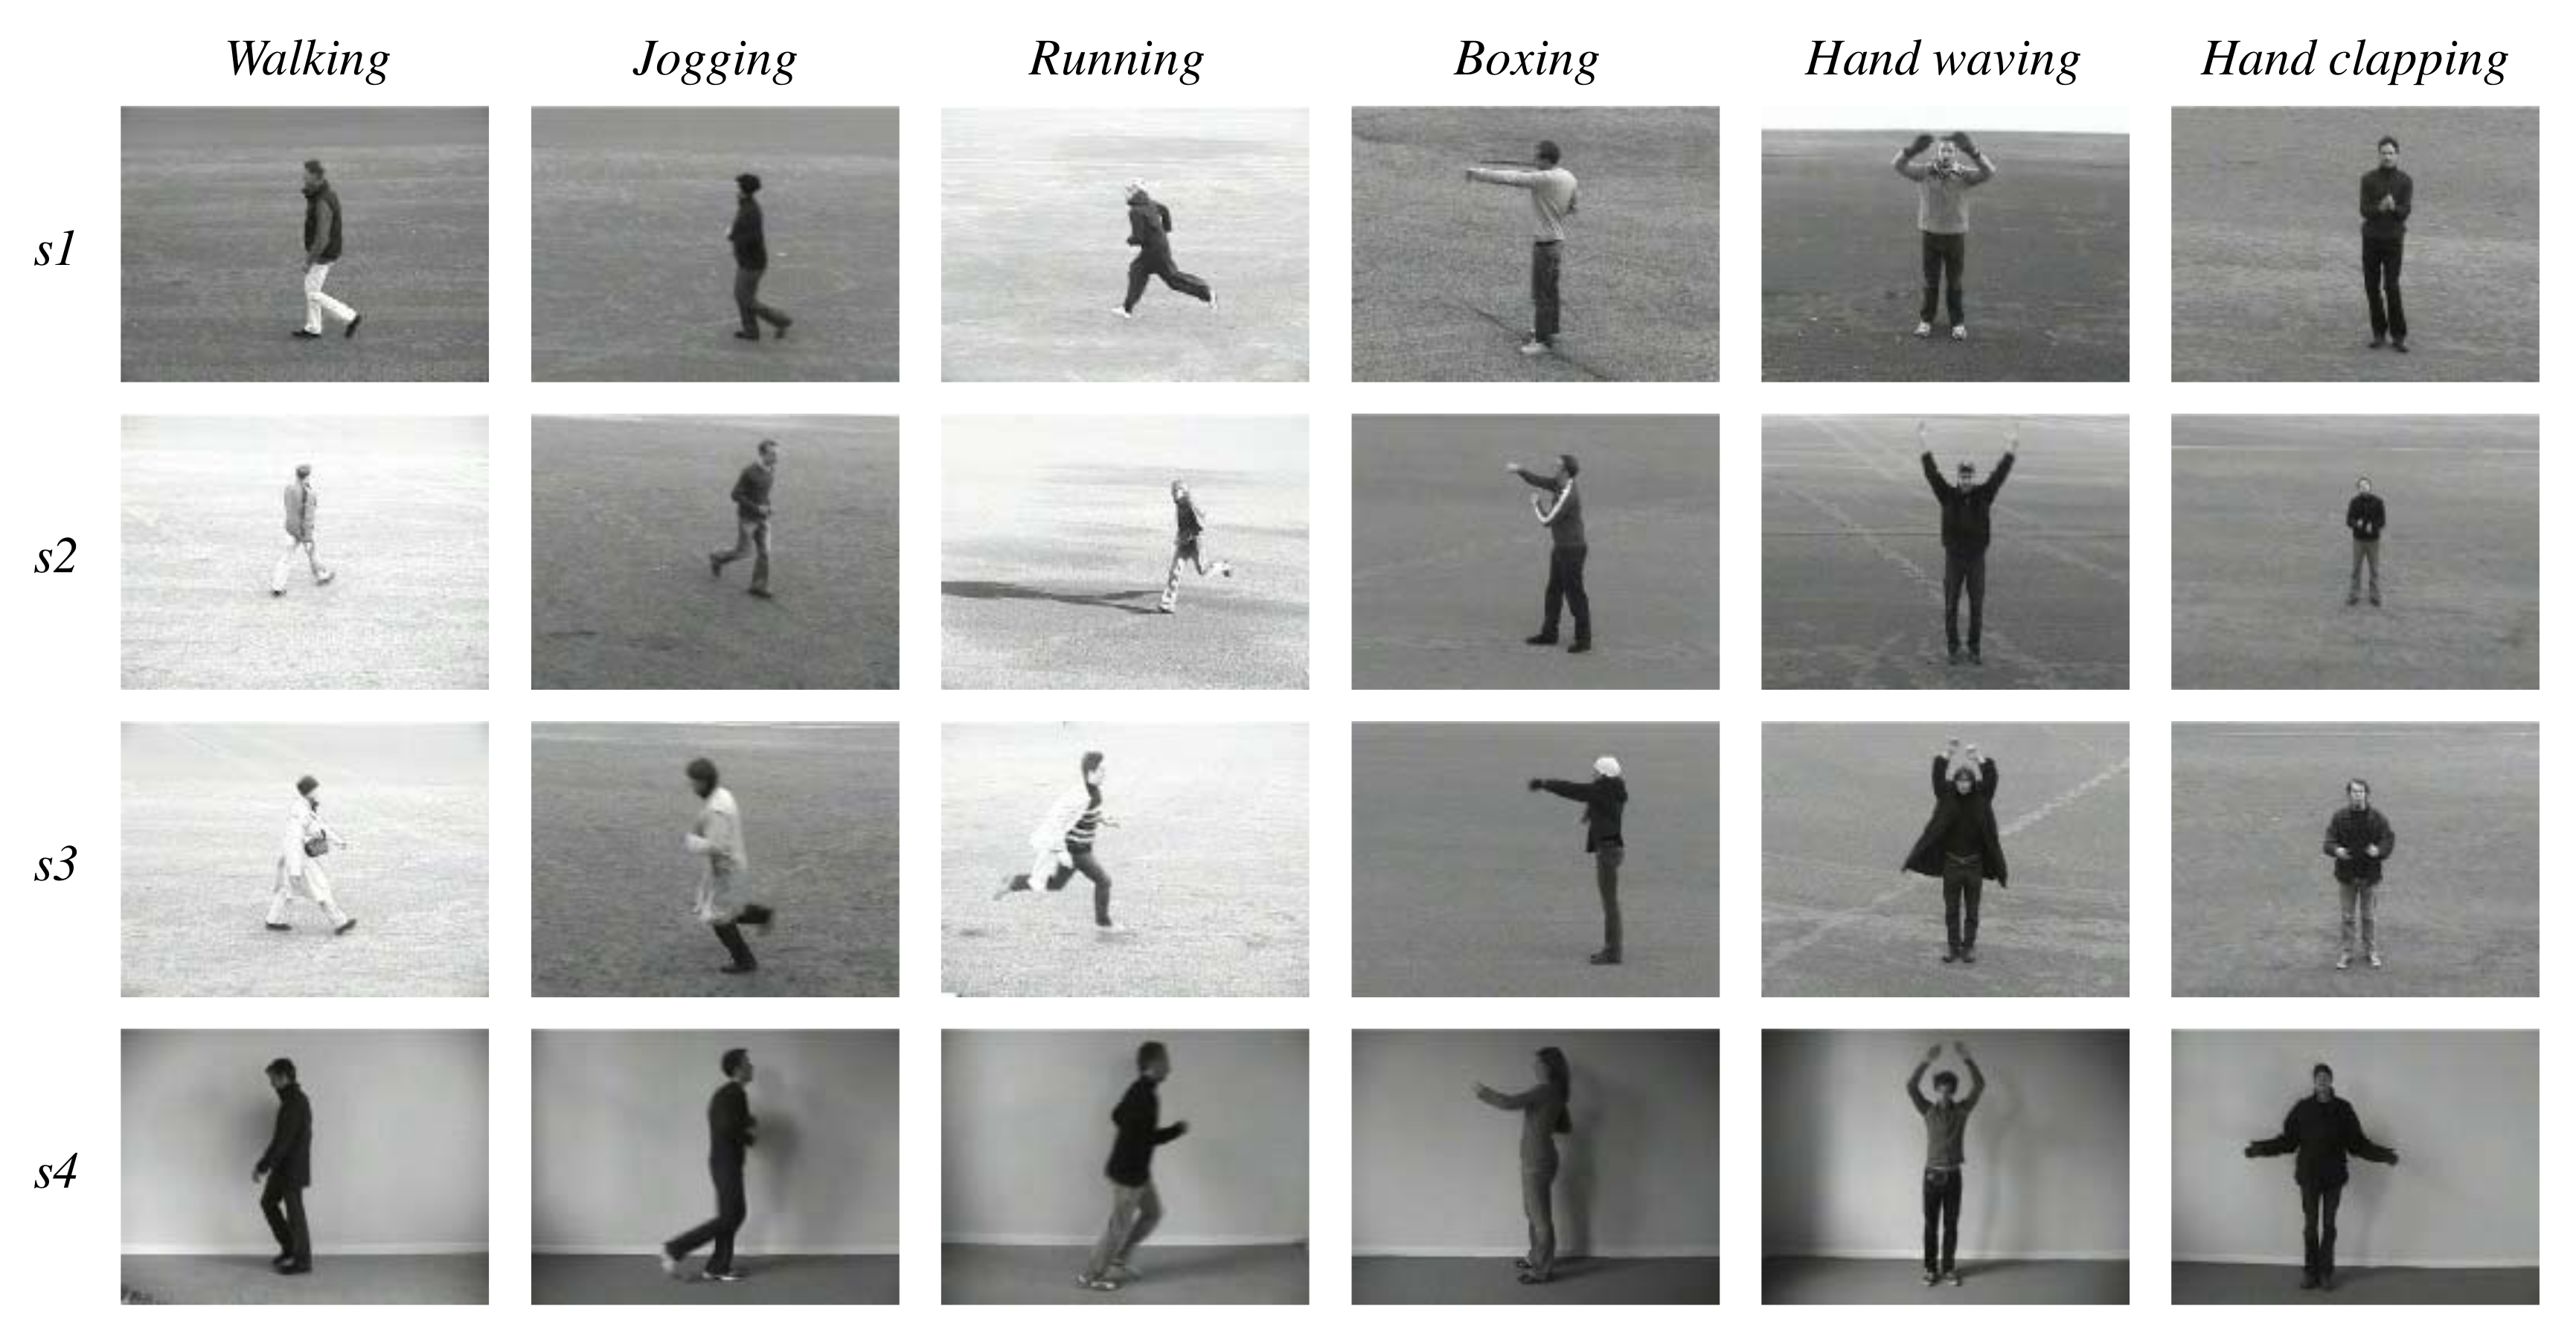
\includegraphics[width=\textwidth]{img_datasets/kth_example}
    \caption{KTH dataset example frames -- 6 different actions classes in 4 different recording scenarios: (s1) outdoors, (s2) outdoors with scale change, (s3) outdoors with chaning clothes, (s4) indoors \cite{schuldt_recognizing_2004}}
    \label{fig:kth_example}
\end{figure}


\subsubsection{Weizmann -- 2005}
%\cite{blank_actions_2005}\\
One year after KTH, the Weizmann dataset \cite{blank_actions_2005} (also known as Weizmann actions as space-time shapes dataset) was released in 2005 by the Weizmann Institute of Science in Israel.
The dataset provides more action classes than KTH but features less performers per action class.
The actions are also recorded in controlled conditions.
Additional to the action labels, the silhouettes of the actors as well as the background sequences for background subtraction are provided with the dataset.
The actors move horizontally in the scene, so no change of their size due to changing distances to the camera is present.
Some actions are repeated in different directions to account for their asymmetrical nature.

Dataset details: \cite{kang_review_2016}
\begin{itemize}
    \item $90$ video clips, each containing multiple instances of a given action class.
    \item $10$ action classes (run, walk, skip, jumping-jack, jump-forward-on-two-legs, jump-in-place-on-two-legs, gallop sideways, wave-two-hands, wave-one-hand and bend) 
    \item $9$ different actors.
    \item Homogeneous, uncluttered backgrounds.
    \item Static camera.
    \item $180 \times 144$ pixels video-resolution @ $25$\textit{fps}.
    \item $3.66s$ average clip length.
\end{itemize}

Figure \ref{fig:weizmann_example} shows example frames for some of the action classes of Weizmann dataset.

\begin{figure}[H]
    \centering
    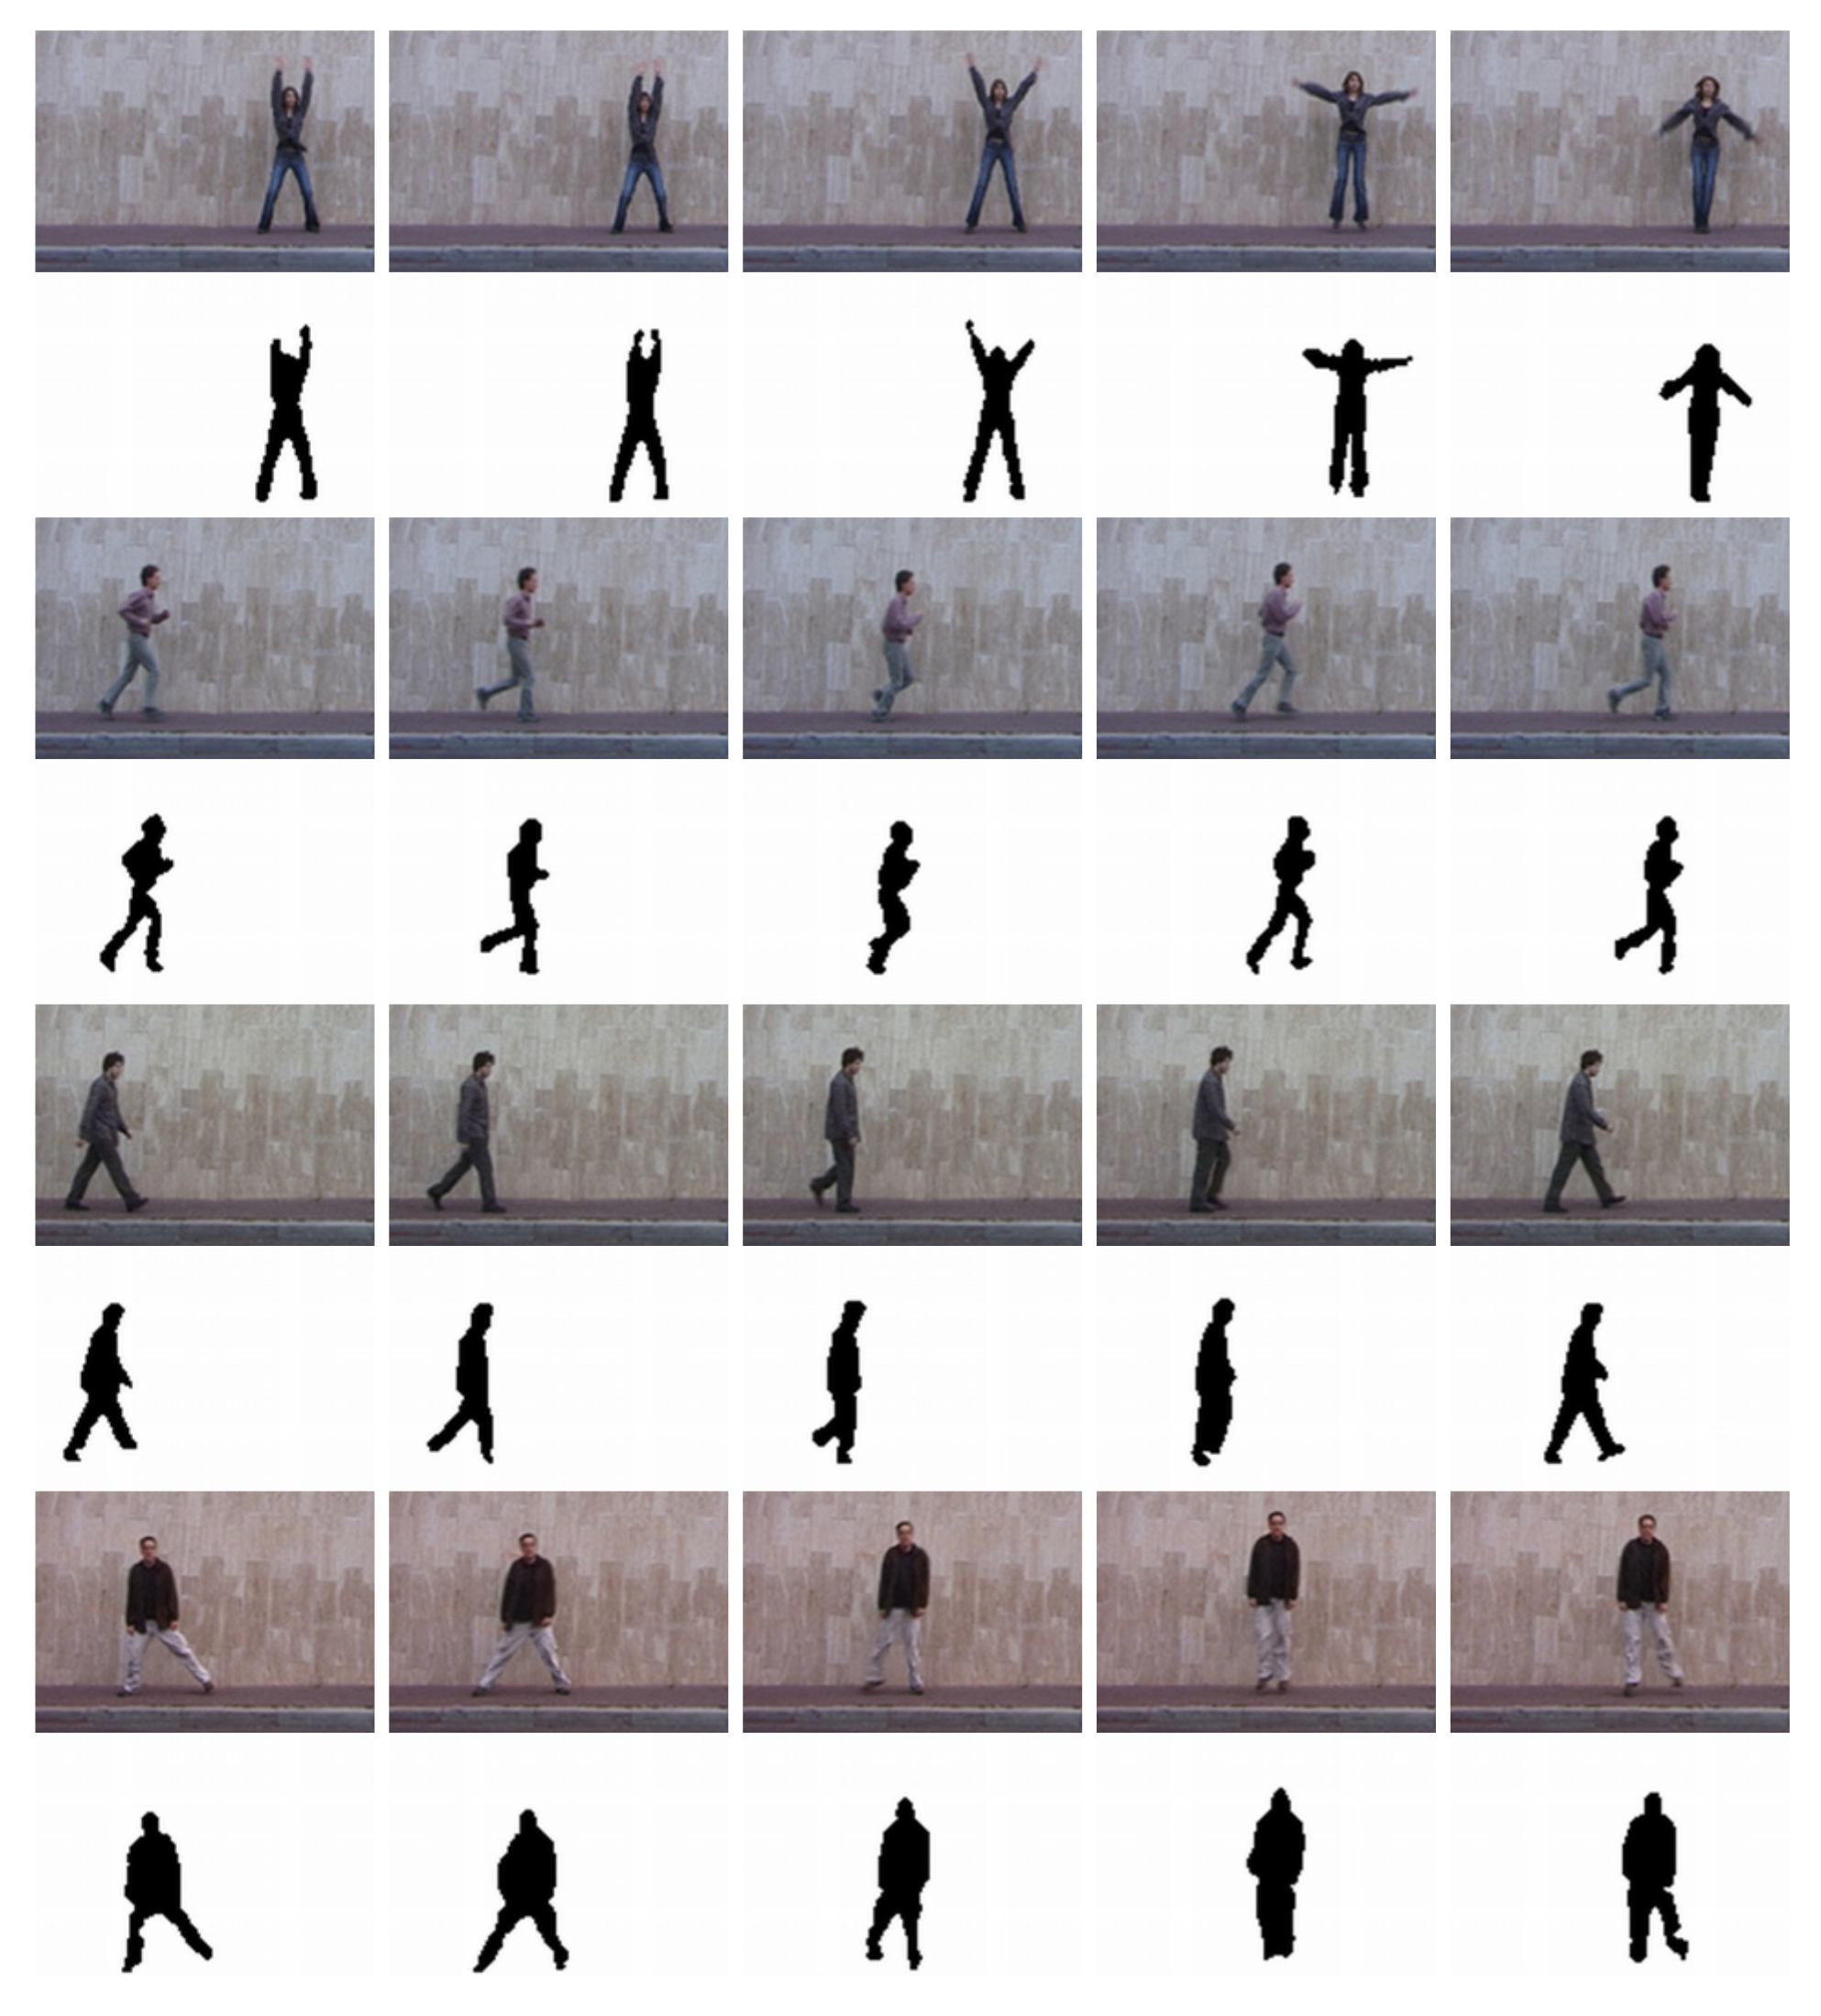
\includegraphics[width=0.7\textwidth]{img_datasets/weizmann_example}
    \caption{Example frames for the action classes \textit{jumping jacks}, \textit{run}, \textit{walk} and \textit{gallop sideways} along with provided foreground silhouette-masks \cite{blank_actions_2005}}
    \label{fig:weizmann_example}
\end{figure}


\subsubsection{IXMAS -- 2006}
%\cite{weinland_free_2006}\\
The INRIA Xmas Motion Acquisition Sequences dataset (IXMAS) \cite{weinland_free_2006} was initially released in 2006 by the French National Institute for Computer Sciences (INRIA) \cite{weinland_free_2006}.
It was designed to study robustness of action recognition algorithms against viewpoint changes, actor gender and body size.
The dataset therefore contains multi-view shots (5 synchronized cameras) of male and female actors performing atomic actions of the daily-living.
The initial release, as described in \cite{weinland_free_2006}, contained $11$ action classes, performed by $10$ actors and was later extended.

Dataset details (extended release): \cite{_inria_????}
\begin{itemize}
    \item $13$ action classes (checking watch, crossing arms, scratching head, sitting down, getting up, turning around, walking, waving, punching, kicking, pointing, picking up, throwing over head and throwing from bottom up).
    \item Each action performed $3$ times by $11$ different actors.
    \item All actions recorded under controlled conditions (indoors).
    \item Homogeneous, uncluttered backgrounds.
    \item Static camera, $5$ different perspectives of each performance.
\end{itemize}

%Example frames of the $11$ actions in the initial release are shown in figure \ref{fig:ixmas_example} below.
Figure \ref{fig:ixmas_fiveviews} shows the five different camera perspectives of the action \textit{checking watch}.
%
%\begin{figure}[H]
%    \centering
%    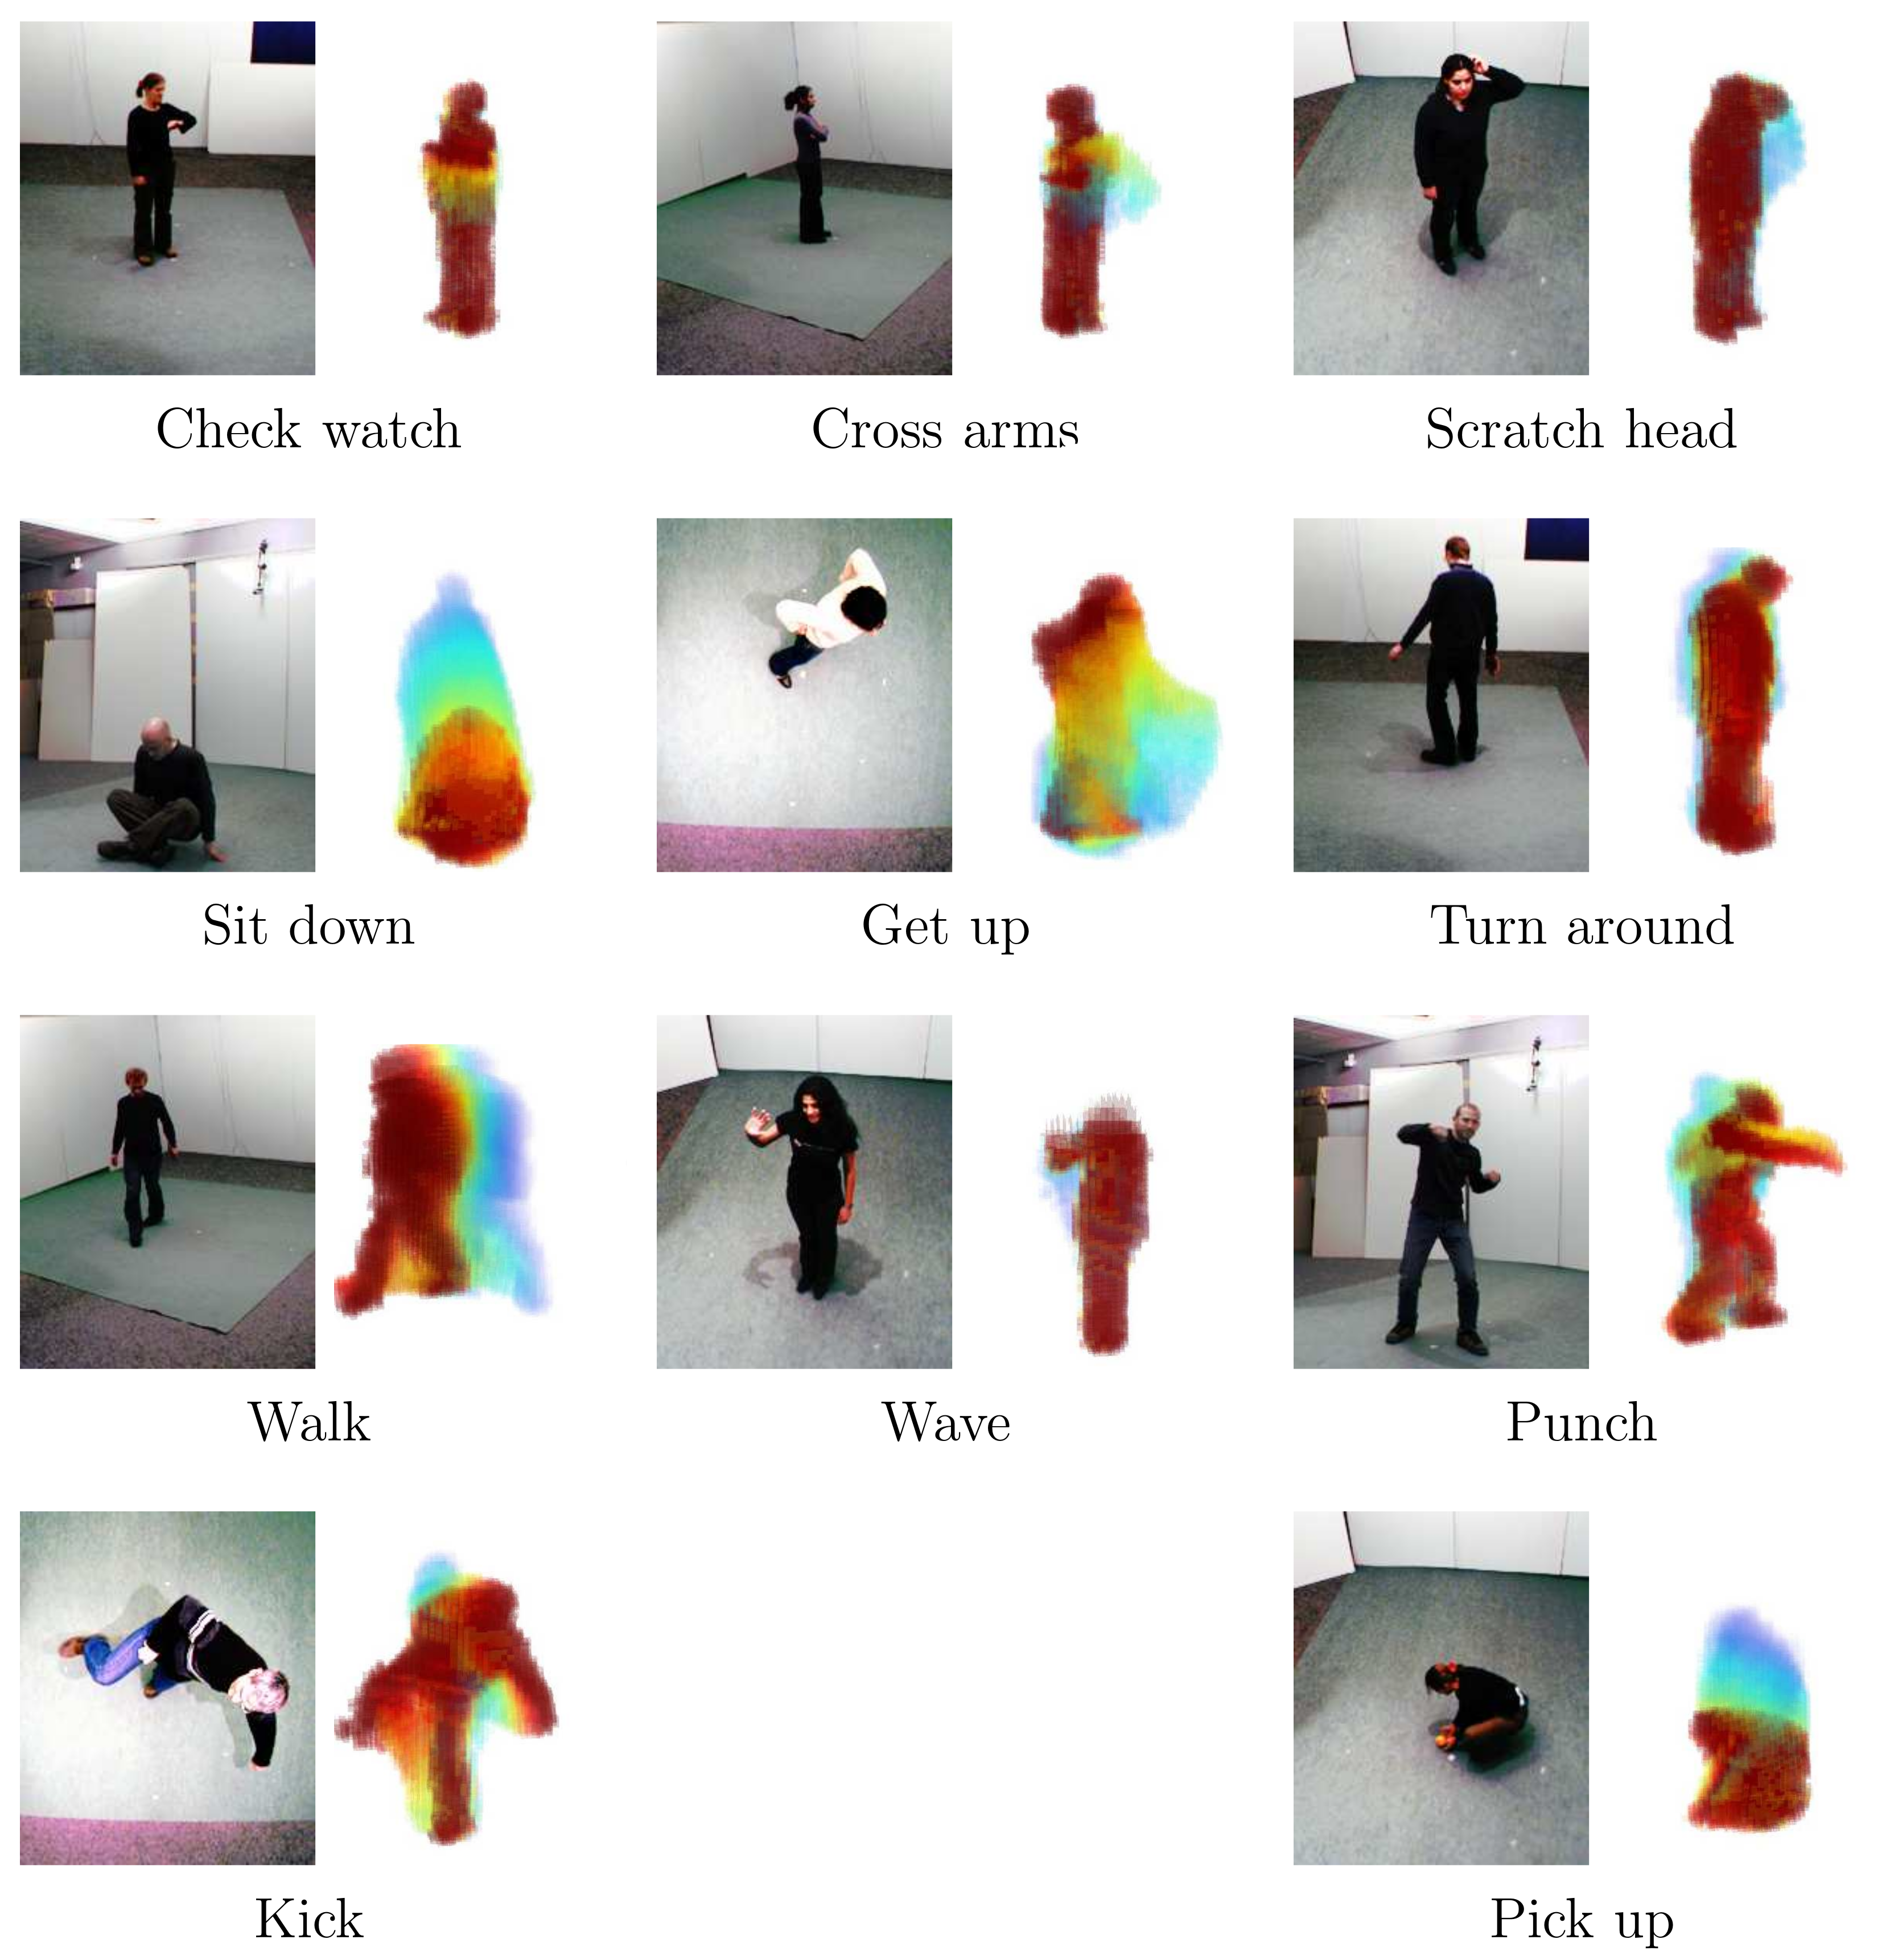
\includegraphics[width=0.8\textwidth]{img_datasets/ixmas_example}
%    \caption{Example frames for the action classes in the initial IXMAS release \cite{weinland_free_2006}}
%    \label{fig:ixmas_example}
%\end{figure}

\begin{figure}[H]
    \centering
    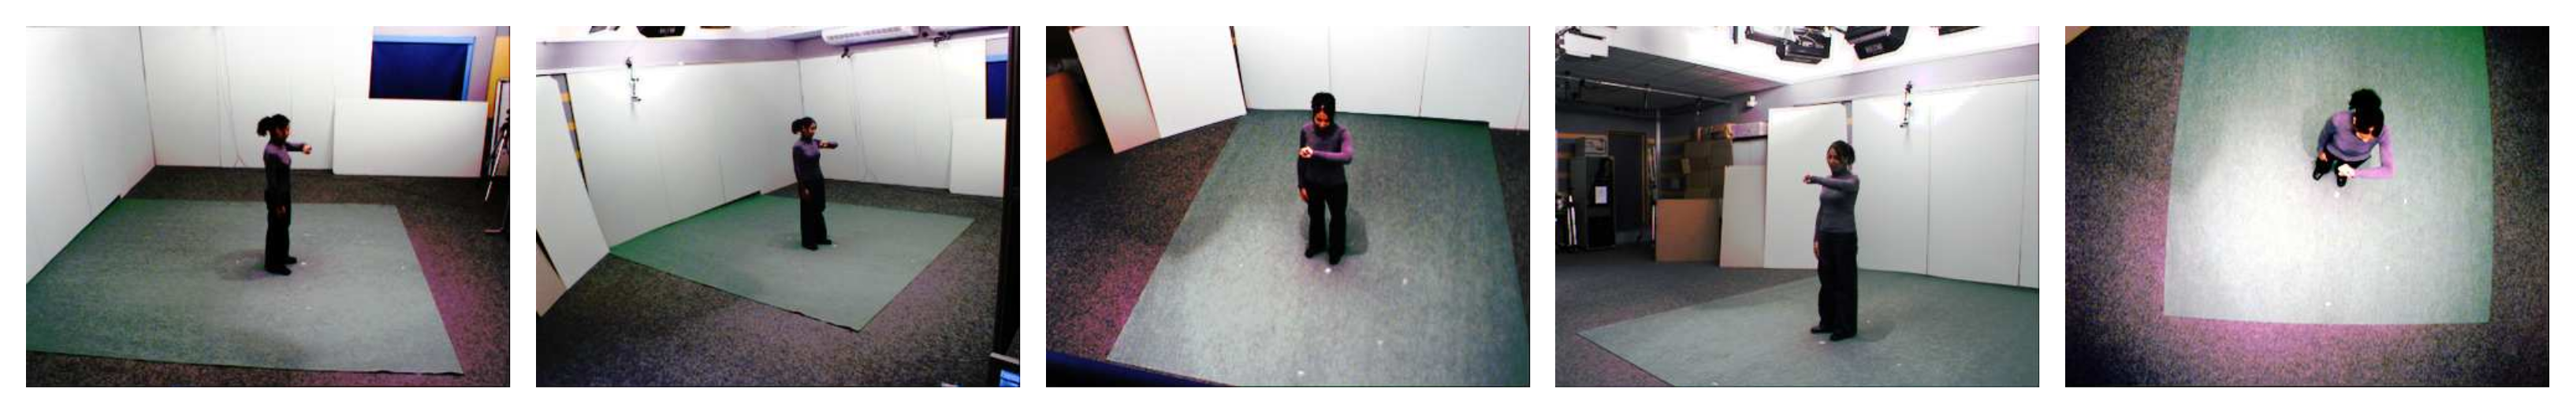
\includegraphics[width=\textwidth]{img_datasets/ixmas_fiveviews}
    \caption{Action example of \textit{checking watch} captured from five different cameras \cite{weinland_free_2006}}
    \label{fig:ixmas_fiveviews}
\end{figure}


\subsection{Intermediate Benchmarking Datasets -- Television and Movies}


\subsubsection{UCF Sports -- 2008}
%\cite{rodriguez_action_2008}\cite{soomro_action_2014}\\
The UCF Sports Dataset was initially released in 2008 by the Department of Electrical Engineering and Computer Science at the University of Central Florida (UCF), where several human action datasets stem from as well.
The dataset contains video clips of sport actions, recorded from broadcast television channels such as the BBC and ESPN.
Because of its origin in television, the video data is of professional quality with moving cameras and changing backgrounds.

The initial release of the dataset \cite{rodriguez_action_2008} contained nine action classes: diving, golf swining, kicking, lifting, horseback riding, running, skating, swinging a baseball bat and pole vaulting
Example frames of the first release are shown in figure \ref{fig:ucfsports1_example}.
For a second release \cite{soomro_action_2014} pole vaulting as well as swinging a baseball bat have been removed and the additional classes swinging on a bench, swinging on parallel bars and walking have been added.
Example frames of the second release are shown in figure \ref{fig:ucfsports2_example}.

Dataset details (second, final release): \cite{_center_????}
\begin{itemize}
    \item $150$ action clips.
    \item $10$ action classes.
    \item Moving camera and changing backgrounds.
    \item $720 \times 480$ pixels video-resolution @ $10$ \textit{fps}.
    \item $6.39s$ average clip length.
    \item $6$ to $22$ clips per class.
\end{itemize}

\begin{figure}[H]
    \centering
    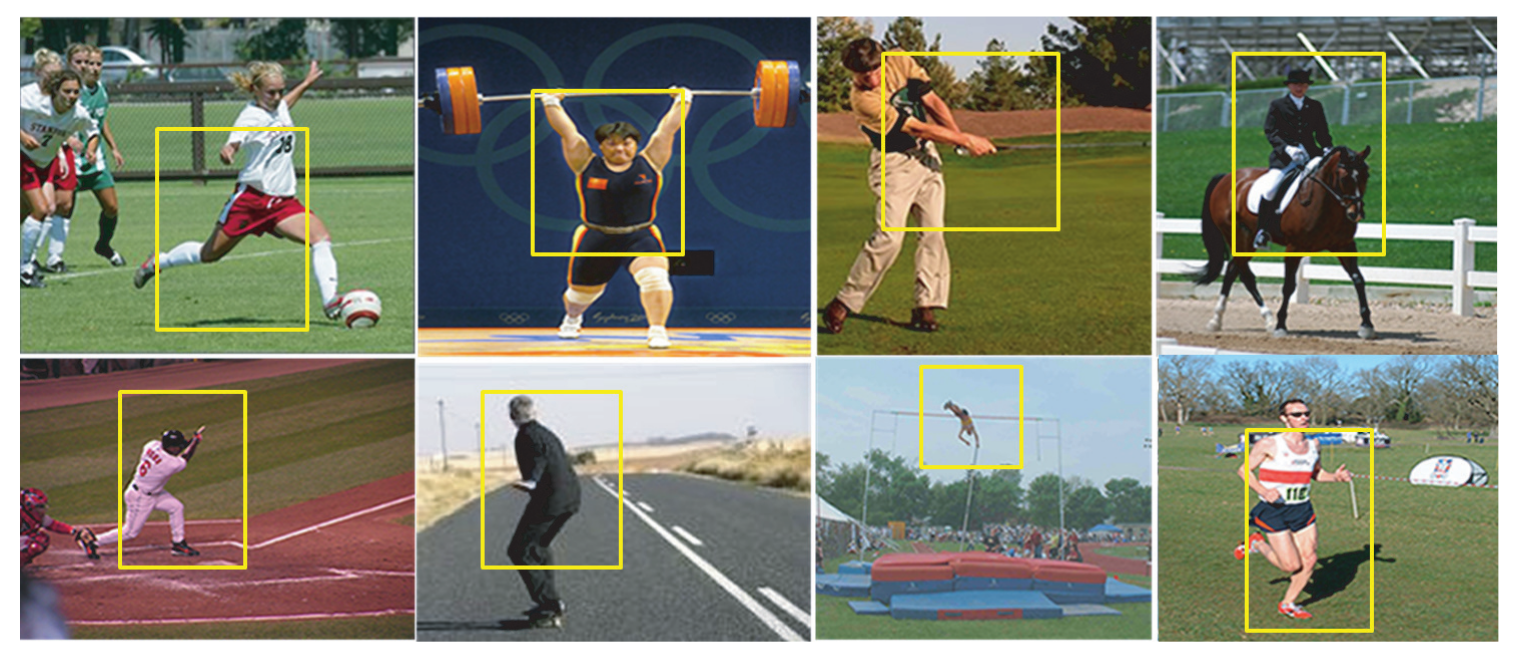
\includegraphics[width=0.9\textwidth]{img_datasets/ucfsports1_example}
    \caption{Example frames of UCF Sports Dataset (release 1) \cite{rodriguez_action_2008}}
    \label{fig:ucfsports1_example}
\end{figure}

\begin{figure}[H]
    \centering
    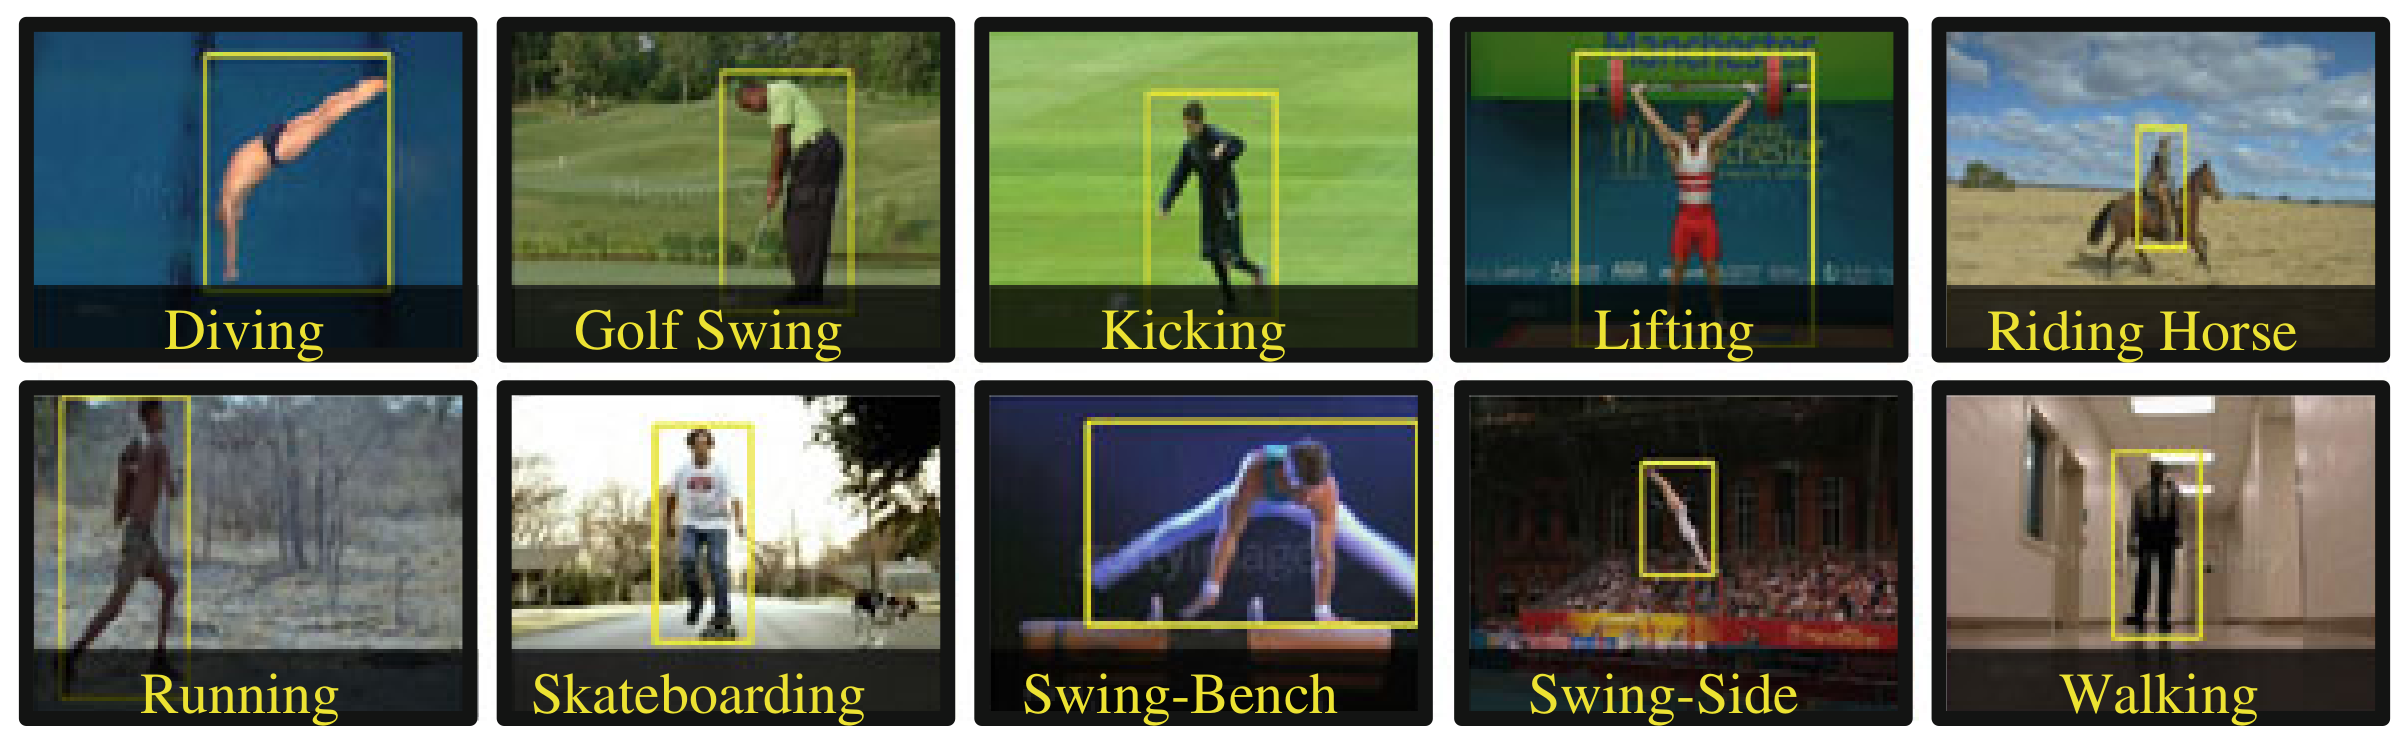
\includegraphics[width=\textwidth]{img_datasets/ucfsports2_example}
    \caption{Example frames of UCF Sports Dataset (release 2) \cite{soomro_action_2014}}
    \label{fig:ucfsports2_example}
\end{figure}


\subsubsection{Hollywood -- 2008}
%\cite{laptev_learning_2008} \\
The Hollywood dataset \cite{laptev_learning_2008} was released in 2008 at the IRISA Institue in France and contains video samples of human actions from $32$ movies, divided into $8$ different action classes.
The dataset provides a predefined split into training and test set.
The test set contains $211$ video samples from $20$ movies.
Two differently annotated training sets with action samples from the remaining $12$ movies are provided.
The \textit{automatic training set} contains $233$ action samples, which are automatically annotated by extracting action labels from the movie scripts.
The labels are approximately 60\% correct.
The \textit{clean training set} contains $219$ action samples with manually verified labels.

The Hollywood dataset and its successor Hollywood 2 are considered more challenging than the previously introduced datasets for benchmarking \cite{chaquet_survey_2013}.
Since the action clips are sampled from movies, the dataset provides a wide range of variation in persons, gestures, clothing, camera motion, perspective and occlusion.
However, since all footage was filmed under controlled lighting conditions with professional cameras, the datasets are considered not representative for real-world observations \cite{kang_review_2016}.

Dataset details: \cite{_ivan_????}
\begin{itemize}
    \item $233 + 219 + 211$ action clips (automatic training set + clean training set + test set)
    \item $8$ action classes (AnswerPhone, GetOutCar, HandShake, HugPerson, Kiss, SitDown, SitUp and StandUp)
    \item $240$ pixels video-height with varying width @ $24$ \textit{fps} 
\end{itemize}

Example frames for all classes of the Hollywood dataset are shown in figure \ref{fig:hollywood1_example}.

\begin{figure}[H]
    \centering
    \includegraphics[width=\textwidth]{img_datasets/hollywood1_example}
    \caption{Example frames for the eight classes of Hollywood I dataset with highest confidence for true/false positives/negatives \cite{laptev_learning_2008}}
    \label{fig:hollywood1_example}
\end{figure}


\subsubsection{Hollywood 2 -- 2009}
%\cite{marszalek_actions_2009}\\
The Hollywood 2 dataset \cite{marszalek_actions_2009} is an extension of the Hollywood dataset and was released in 2009 at the IRISA Institute of France.
Besides adding $4$ action classes to the Hollywood dataset, Hollywood 2 contains $10$ classes of indoor and outdoor scenes to study if action recognition algorithms benefit from correlating scenes and actions.
The dataset contains $12$ classes of human actions, $10$ classes of scenes and features approximately $20.1$ hours of video in total from $69$ movies.
Equivalently to Hollywood 1, automatically and manually verified labels are provided in two training sets.

Dataset details (action clips): \cite{_ivan_????-1}
\begin{itemize}
    \item $810 + 823 + 882$ action clips (automatic + clean training set + test set)
    \item $12$ action classes (AnswerPhone, GetOutCar, HandShake, HugPerson, Kiss, SitDown, SitUp, StandUp, Eat, FightPerson, Run, DriveCar)
\end{itemize}

Figure \ref{fig:hollywood2_example} shows the additional classes in the Hollywood 2 datasets.

\begin{figure}[H]
    \centering
    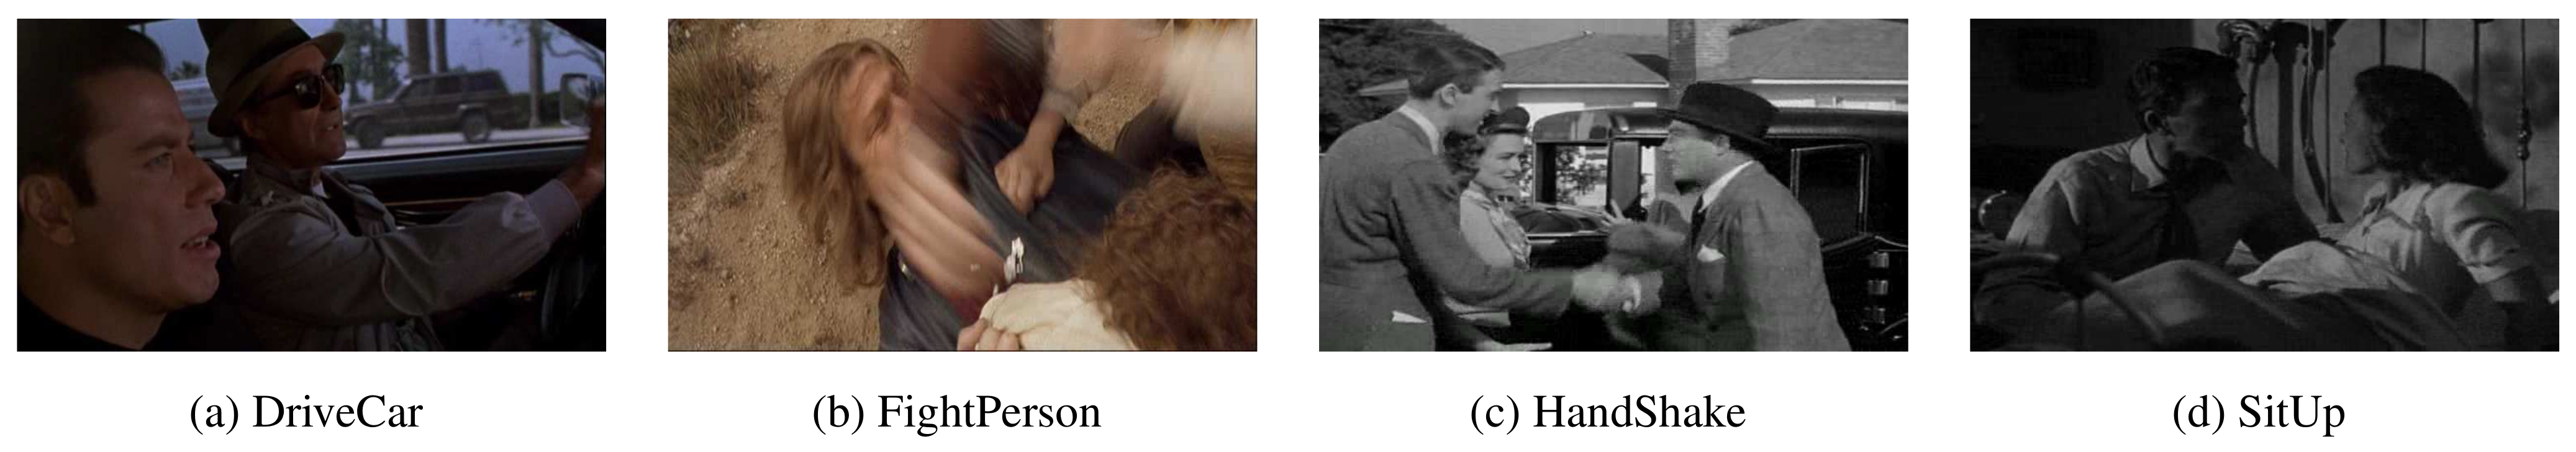
\includegraphics[width=\textwidth]{img_datasets/hollywood2_example}
    \caption{Example frames for the additional classes of Hollywood 2 dataset \cite{marszalek_actions_2009}}
    \label{fig:hollywood2_example}
\end{figure}


\subsection{Modern Benchmarking Datasets -- Videos in the Wild}

\subsubsection{UCF11 Youtube Action -- 2009}
%\cite{liu_recognizing_2009}\\
The UCF11 dataset \cite{liu_recognizing_2009}, also known as UCF YouTube Action dataset, was released in 2009 by the University of Central Florida (UCF).
It contains videos from YouTube in $11$ action classes.
Since the authors were not involved in the video recognition process, the dataset features a variety of different conditions in the videos: a mix of shaky and steady cameras, different (cluttered) backgrounds, people shown in different scales, varying illumination and low resolution.
There are several releases of the dataset, here properties of the last release are reported.

Dataset details: \cite{_center_????-1}
\begin{itemize}
    \item $1600$ action clips.
    \item $11$ action classes: basketball shooting, biking/cycling, diving, golf swinging, horse back riding, soccer juggling, swinging, tennis swinging, trampoline jumping, volleyball spiking, and walking with a dog.
    \item Varying spatial resolution (max. $240 \times 320$ pixels) @ 29\textit{fps}.
    \item Clip length between $22$ and $900$ frames.
\end{itemize}

Figure \ref{fig:ucfyoutube_example} shows example frames of the dataset.

\begin{figure}[H]
    \centering
    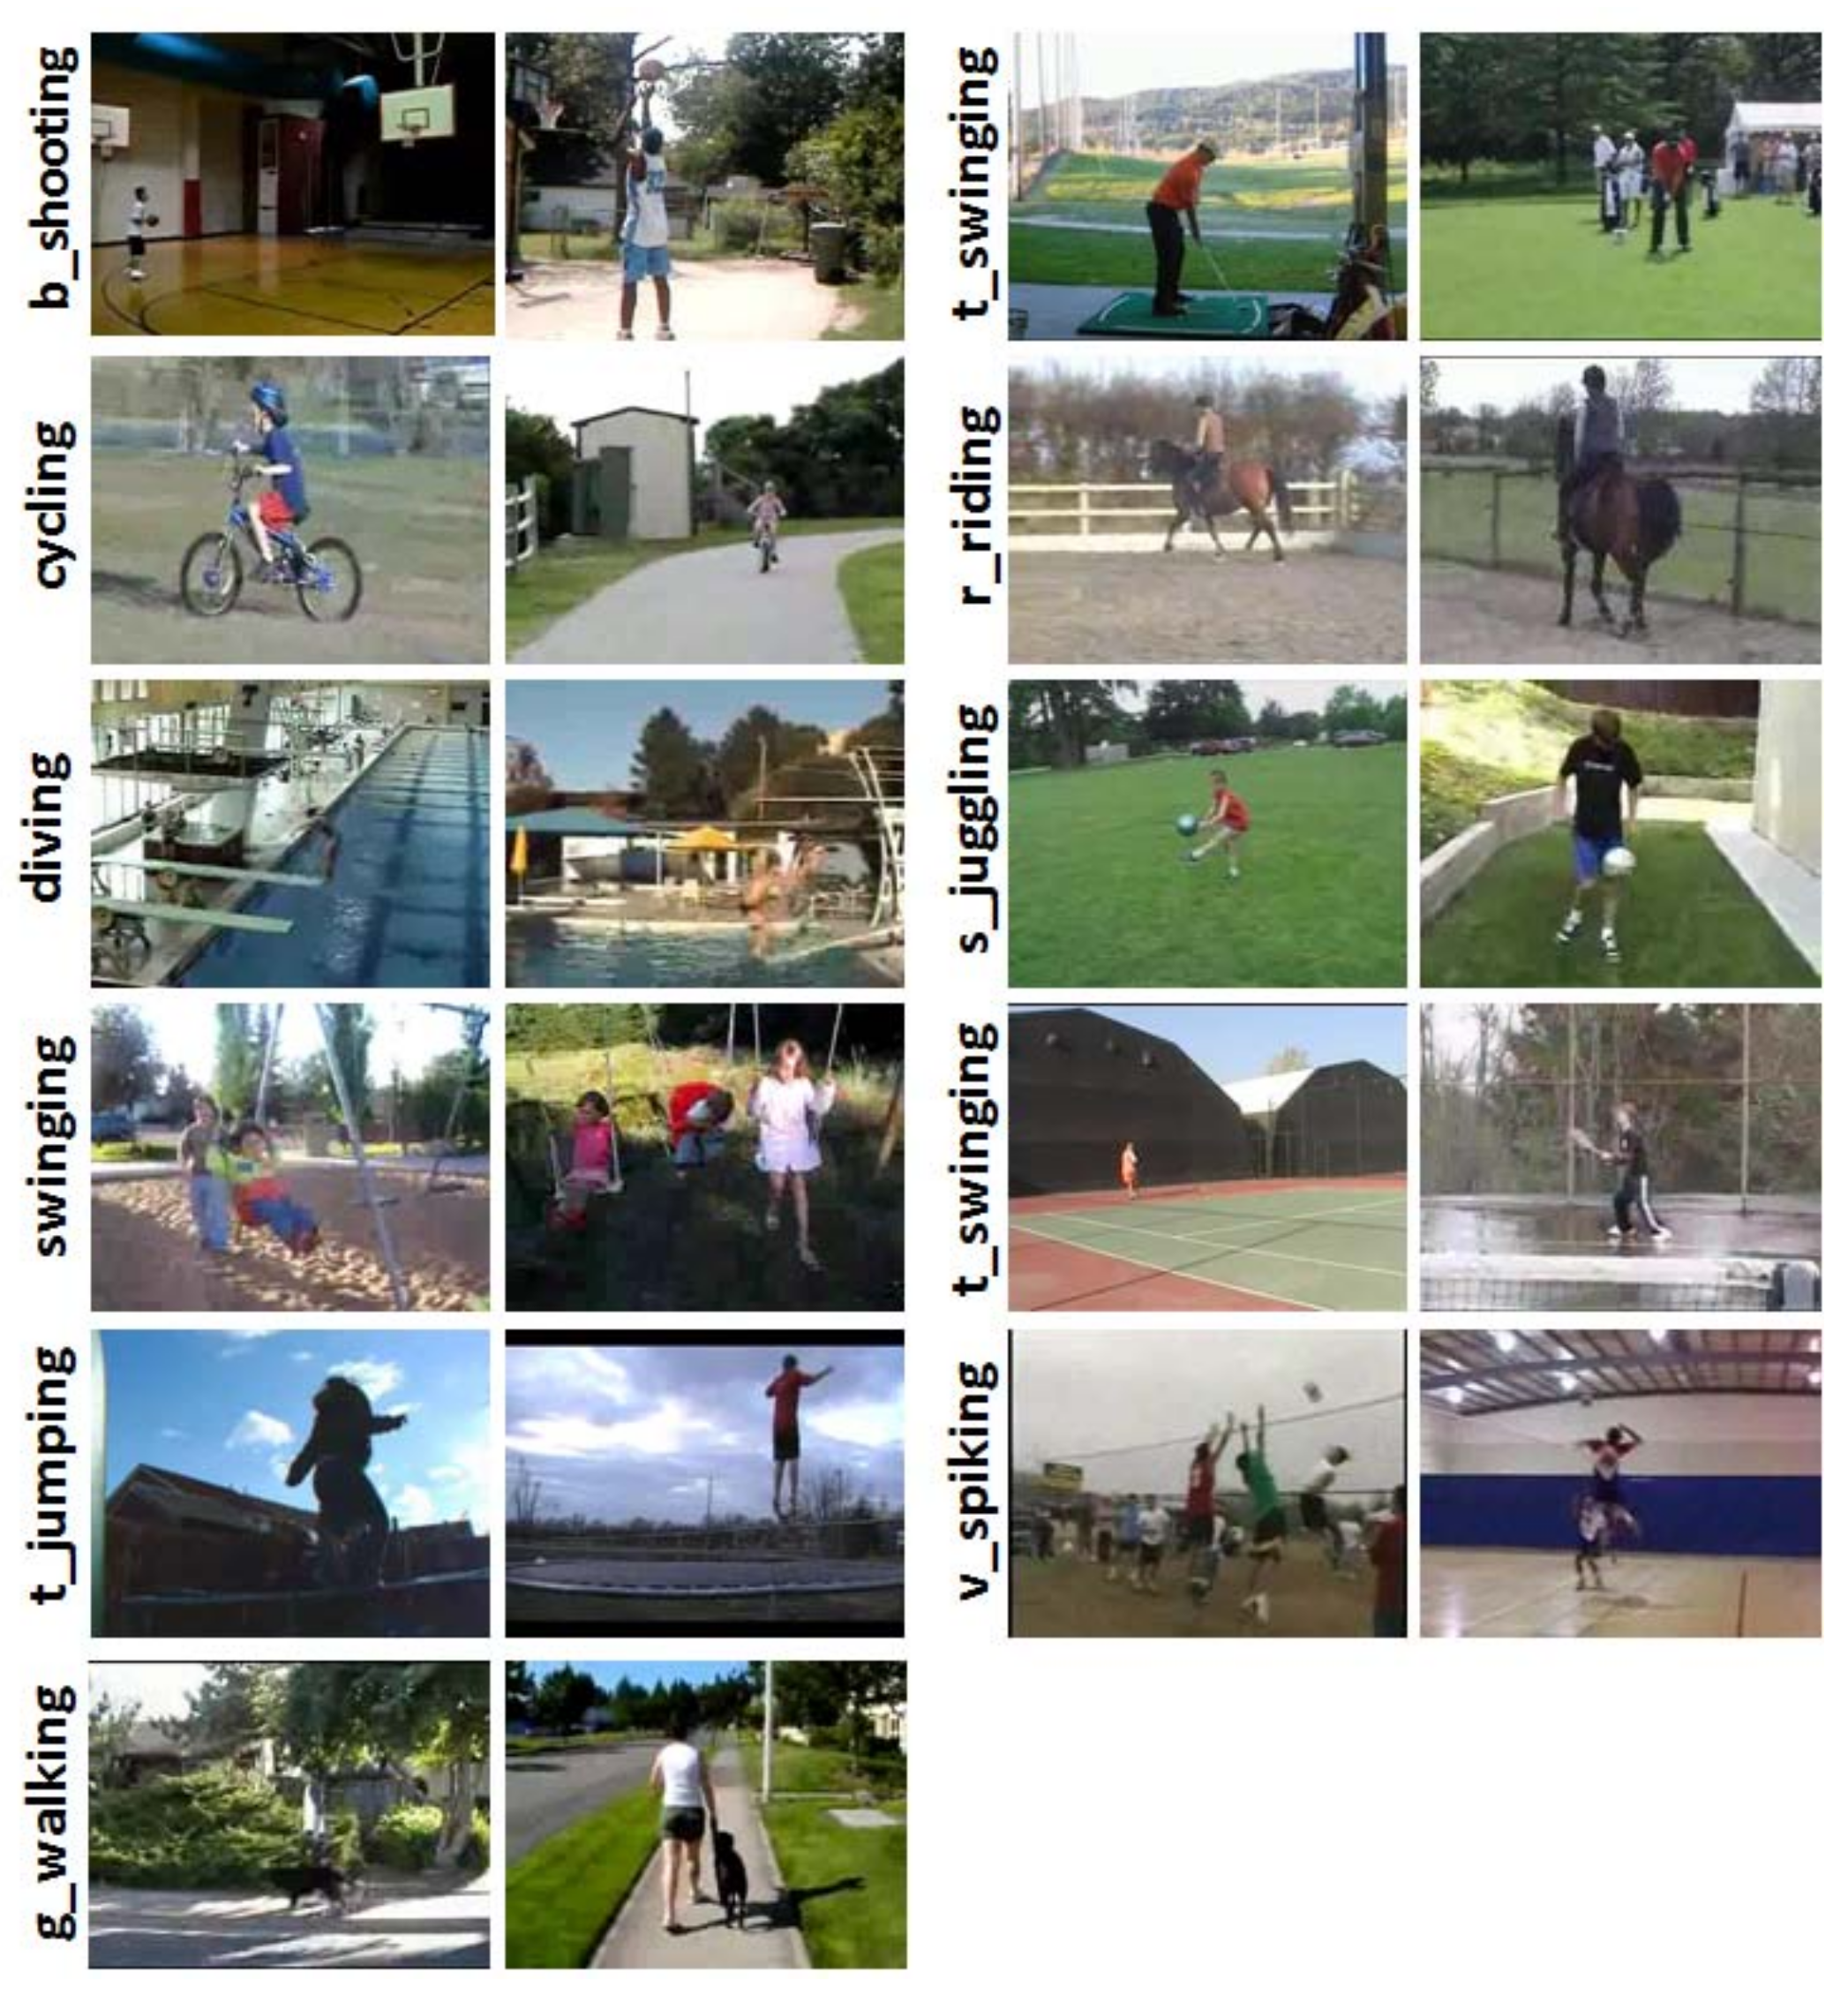
\includegraphics[width=.7\textwidth]{img_datasets/ucfyoutube_example}
    \caption{Example frames of the 11 classes in the UCF YouTube actions dataset \cite{liu_recognizing_2009}}
    \label{fig:ucfyoutube_example}
\end{figure}


\subsubsection{UCF50 -- 2010}
%\cite{reddy_recognizing_2013}\\
The UCF50 dataset \cite{reddy_recognizing_2013} is an extension of the UCF11 dataset and was released by the University of Central Florida (UCF) in 2010.
It adds $39$ action classes to UCF11, which results in a total of $50$ action classes.

Dataset details: \cite{kang_review_2016}
\begin{itemize}
    \item $6,676$ action clips.
    \item $50$ action classes (see figure \ref{fig:ucf50_example}).
    \item At least $100$ clips per class.
    \item $320 \times 240$ pixels video-resolution.
\end{itemize}

\begin{figure}[H]
    \centering
    \includegraphics[width=\textwidth]{img_datasets/ucf50_example}
    \caption{Example frames of the 50 classes in UCF50 \cite{reddy_recognizing_2013}}
    \label{fig:ucf50_example}
\end{figure}


\subsubsection{HMDB51 -- 2011}
%\cite{kuehne_hmdb:_2011}
The Human Motion Database (HMDB51) \cite{kuehne_hmdb:_2011} was created by the Brown University in the USA and was released in 2011.
The HMDB51 dataset consists of $6,849$ action clips in $51$ classes sampled mostly from movies, public video databases and YouTube.
Each action class contains a minimum of $101$ action clips.
The source videos presented different resolutions and frame rates.
To maintain consistency throughout the dataset, the authors scaled the videos to provide a frame-heigth of $240$ pixels and the width was scaled accordingly.
The framerate of all videos was converted to $30$ \textit{fps}.

Each video of the dataset contains one action but the exact temporal location of the action is not provided.
However, additionally to the action labels, the datasets provides detailed meta information to each action clip: \cite{_serre_????}
\begin{itemize}
    \item Visible body parts: Head, upper body, full body, lower body.
    \item Camera motion: Motion, static.
    \item Camera viewpoint: Front, back, left, right.
    \item Number of people involved in the action: Single, two, three.
    \item Video quality: good, medium, bad.
\end{itemize}

Global movement caused by camera/background movement interfers with local motion in the scene, which is essential for action recognition.
The authors therefore calculated stabilization mask, which can be used to suppress global motions in the clips up to a certain degree. \cite{kuehne_hmdb:_2011}

The action classes in the datset can be grouped into the following five categories: \cite{kuehne_hmdb:_2011}
\begin{enumerate}
    \item General facial actions (e.g.\ smile, laugh, chew, talk)
    \item Facial actions with object manipulation (e.g.\ smoke, eat, drink)
    \item General body movements (e.g.\ clap hands, climb stairs, jump)
    \item Body movements with object interaction (e.g.\ brush hair, catch, kick ball)
    \item Body movements for human interaction (e.g.\ hug, fencing, kiss)
\end{enumerate}

Figure \ref{fig:hmdb_example} shows example frames for each of the action classes in HMDB51.

\begin{figure}[H]
    \centering
    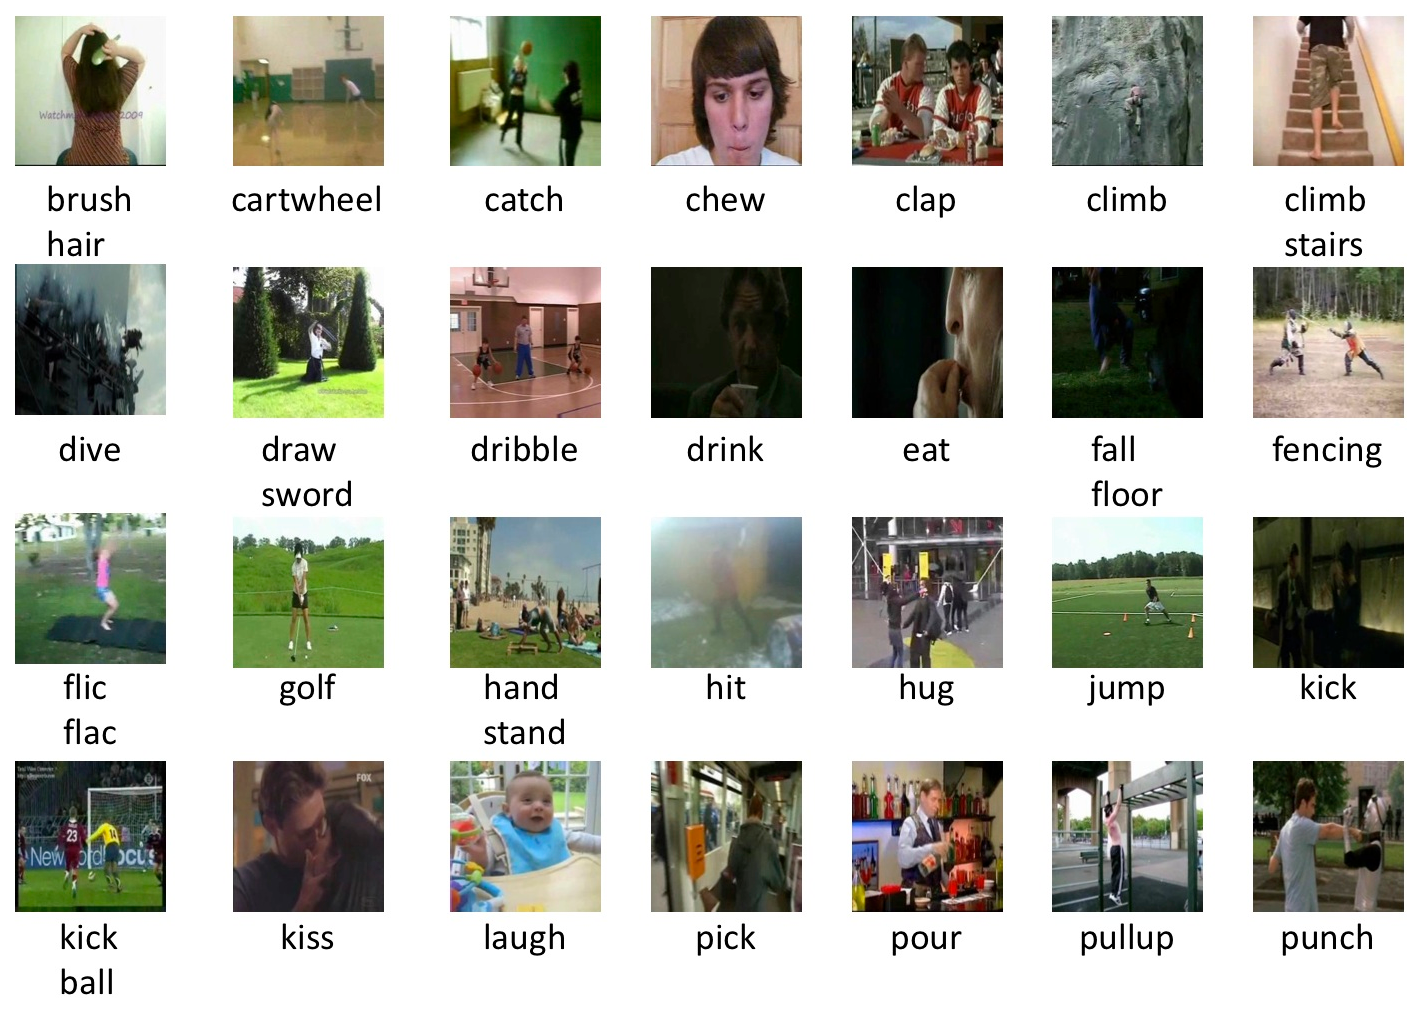
\includegraphics[width=\textwidth]{img_datasets/hmdb_classes1}
    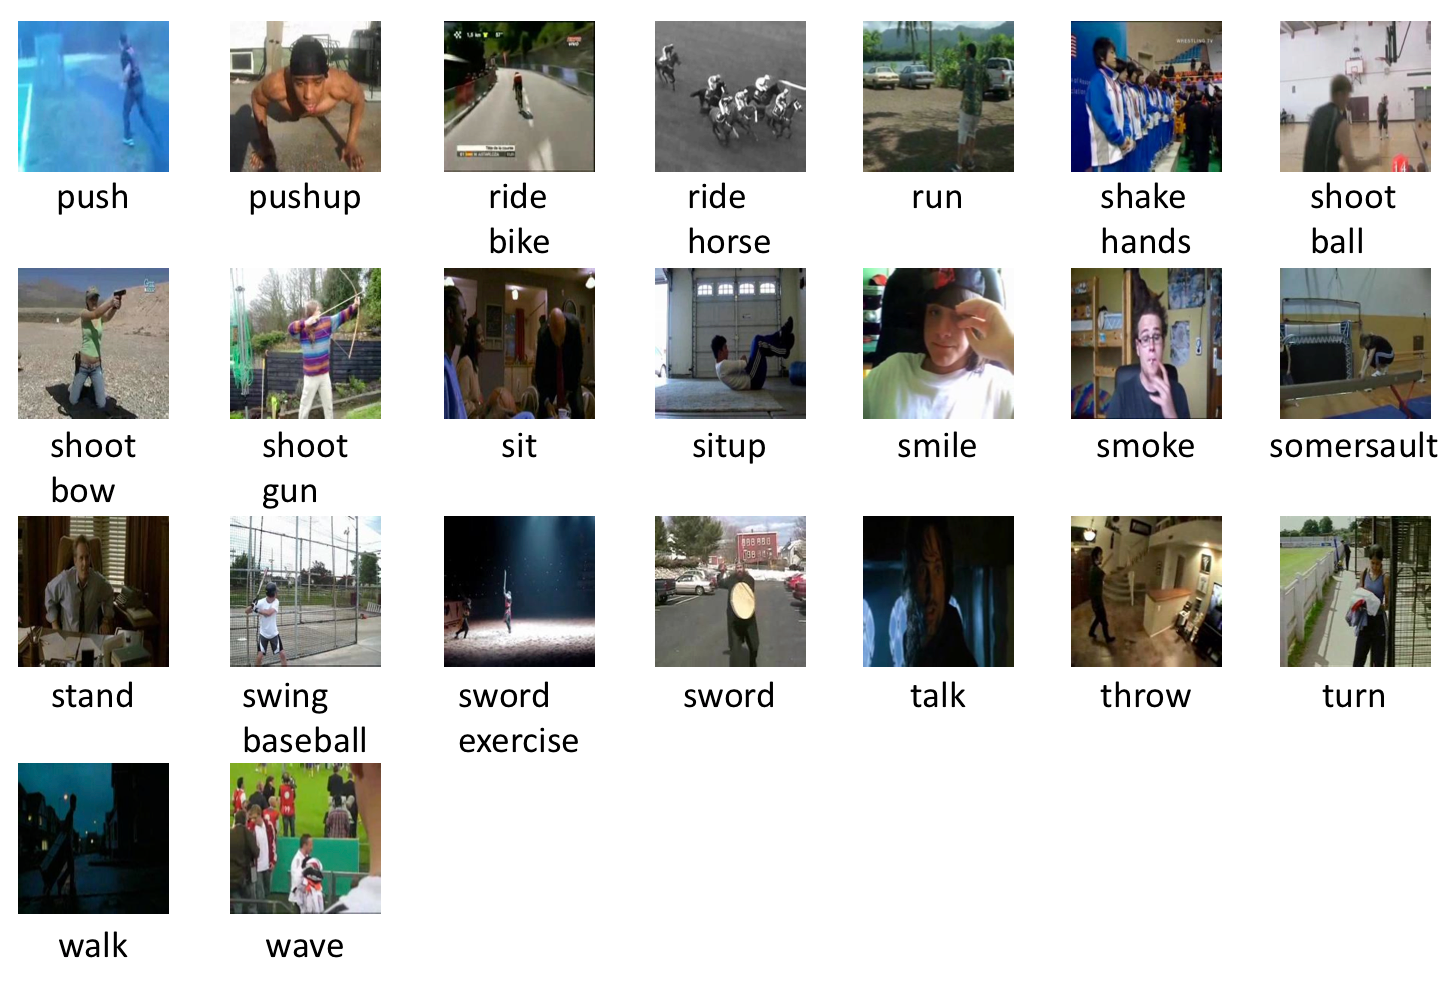
\includegraphics[width=\textwidth]{img_datasets/hmdb_classes2}
    \caption{Example frames for the 51 classes in HMDB51 \cite{_serre_????}}
    \label{fig:hmdb_example}
\end{figure}


\subsubsection{UCF101 -- 2012}
The UCF101 dataset \cite{soomro_ucf101:_2012} is an extension of the UCF50 dataset and was released by the University of Central Florida (UCF) in 2012.
It introduces $51$ additional classes sampled from YouTube videos, which results in a total of $13,320$ action clips in $101$ action classes.
The overall length of the dataset is about $27$ hours, with an average length of $7.21s$ per action clip.
Video clips have a resolution of $320 \times 240$ pixels @ $25$ \textit{fps}. 

Figure \ref{fig:ucf101_example} shows example frames of UCF101.
The action classes can be divided into five categories: \cite{soomro_ucf101:_2012}
\begin{itemize}
    \item Blue: Human-object interaction
    \item Red: Body-motion only
    \item Purple: Human-human interaction
    \item Orange: Playing musical instrument
    \item Green: Sports
\end{itemize}

\begin{figure}
    \centering
    \includegraphics[width=\textwidth]{img_datasets/ucf101_example}
    \caption{Example frames of the 101 classes in UCF101 \cite{soomro_ucf101:_2012}}
    \label{fig:ucf101_example}
\end{figure}


\subsubsection{ASLAN -- 2012}
%\cite{kliper-gross_action_2012} \\
In contrast to the previously presented benchmarking datasets, the \textit{Action Similarity Labeling} collection (ASLAN) \cite{kliper-gross_action_2012} emphasizes on a different evaluation protocoll for benchmarking action recognition performance.
Generally multi-class mean recognition accuracy is used as a performance measure, ASLAN however was designed as binary \textit{same}/\textit{not same} classification benchmark.
Specifically, an algorithm is trained on pairs of action video clips labeled \textit{same}/\textit{not same} and is then evaluated on determining the similarity of two unknown clips, i.e.\ determining if they belong to the same class or not.
Thereby test-set clips are drawn from different action classes as the training-set clips, which means an algorithm is evaluated on never before seen examples of an unknown class.

The authors \textcite{kliper-gross_action_2012} argue, that developing algorithms for measuring the similarity of actions has several advantages:
\begin{enumerate}
    \item It eases the problem of ambiguous action labels for complex actions, i.e.\ complex actions can be composed of multiple atomic actions and therefore have multiple actions labels.
    \item By focusing on action similarity, instead of on features that define certain actions, the benchmark leads an algorithm towards a generalization ability that is not limited by a given set of actions.
    \item The binary nature of the benchmark makes it easier to define tests for a given algorithm.
\end{enumerate}
Additionally, determining the similarity of actions can be used in an own class of applications, e.g.\ when similar clips need to be retrieved autonomously from the internet given a video clip with an unknown action label.

Dataset details: \cite{kliper-gross_action_2012}
\begin{itemize}
    \item $3,631$ unique action instances obtained from YouTube videos.
    \item $432$ action classes, manually labeled.
    \item $8.5$ average samples per class
    \item $316$ classes with more than $1$ action sample.
    \item $71$ long samples (duration > $10s$).
    \item $187$ short sampled (duration < $1s$).
    \item Each clip contains one action, no detection needed.
\end{itemize}

The authors provide two different divisions of their database, wich they call \textit{Views}.

\begin{enumerate}
    \item \textit{View-1} is intended for algorithm development and consists of a training- and testing-set which are mutually exclusive, i.e.\ do not share action classes.
        The training-set consists of $1,200$ video pairs, $600$ of which labeled \textit{same} and $600$ labeled \textit{not same}.
        The testing-set consists of $600$ video pairs, $300$ labeled \textit{same} and $300$ labeled \textit{not same}.
    \item \textit{View-2} is intended for reporting the final accuracy of the classifier and consists of $10$ mutually exclusive splits of the database.
        Each split contains 600 video pairs, $300$ labeled \textit{same} and $300$ labeled \textit{not same}.
\end{enumerate}
The authors advise reporting the final performance of the algorithm by doing 10-fold cross-validation using the splits of \textit{View-2}.

\begin{minipage}[t]{0.4\textwidth}
    \begin{figure}[H]
        \centering
        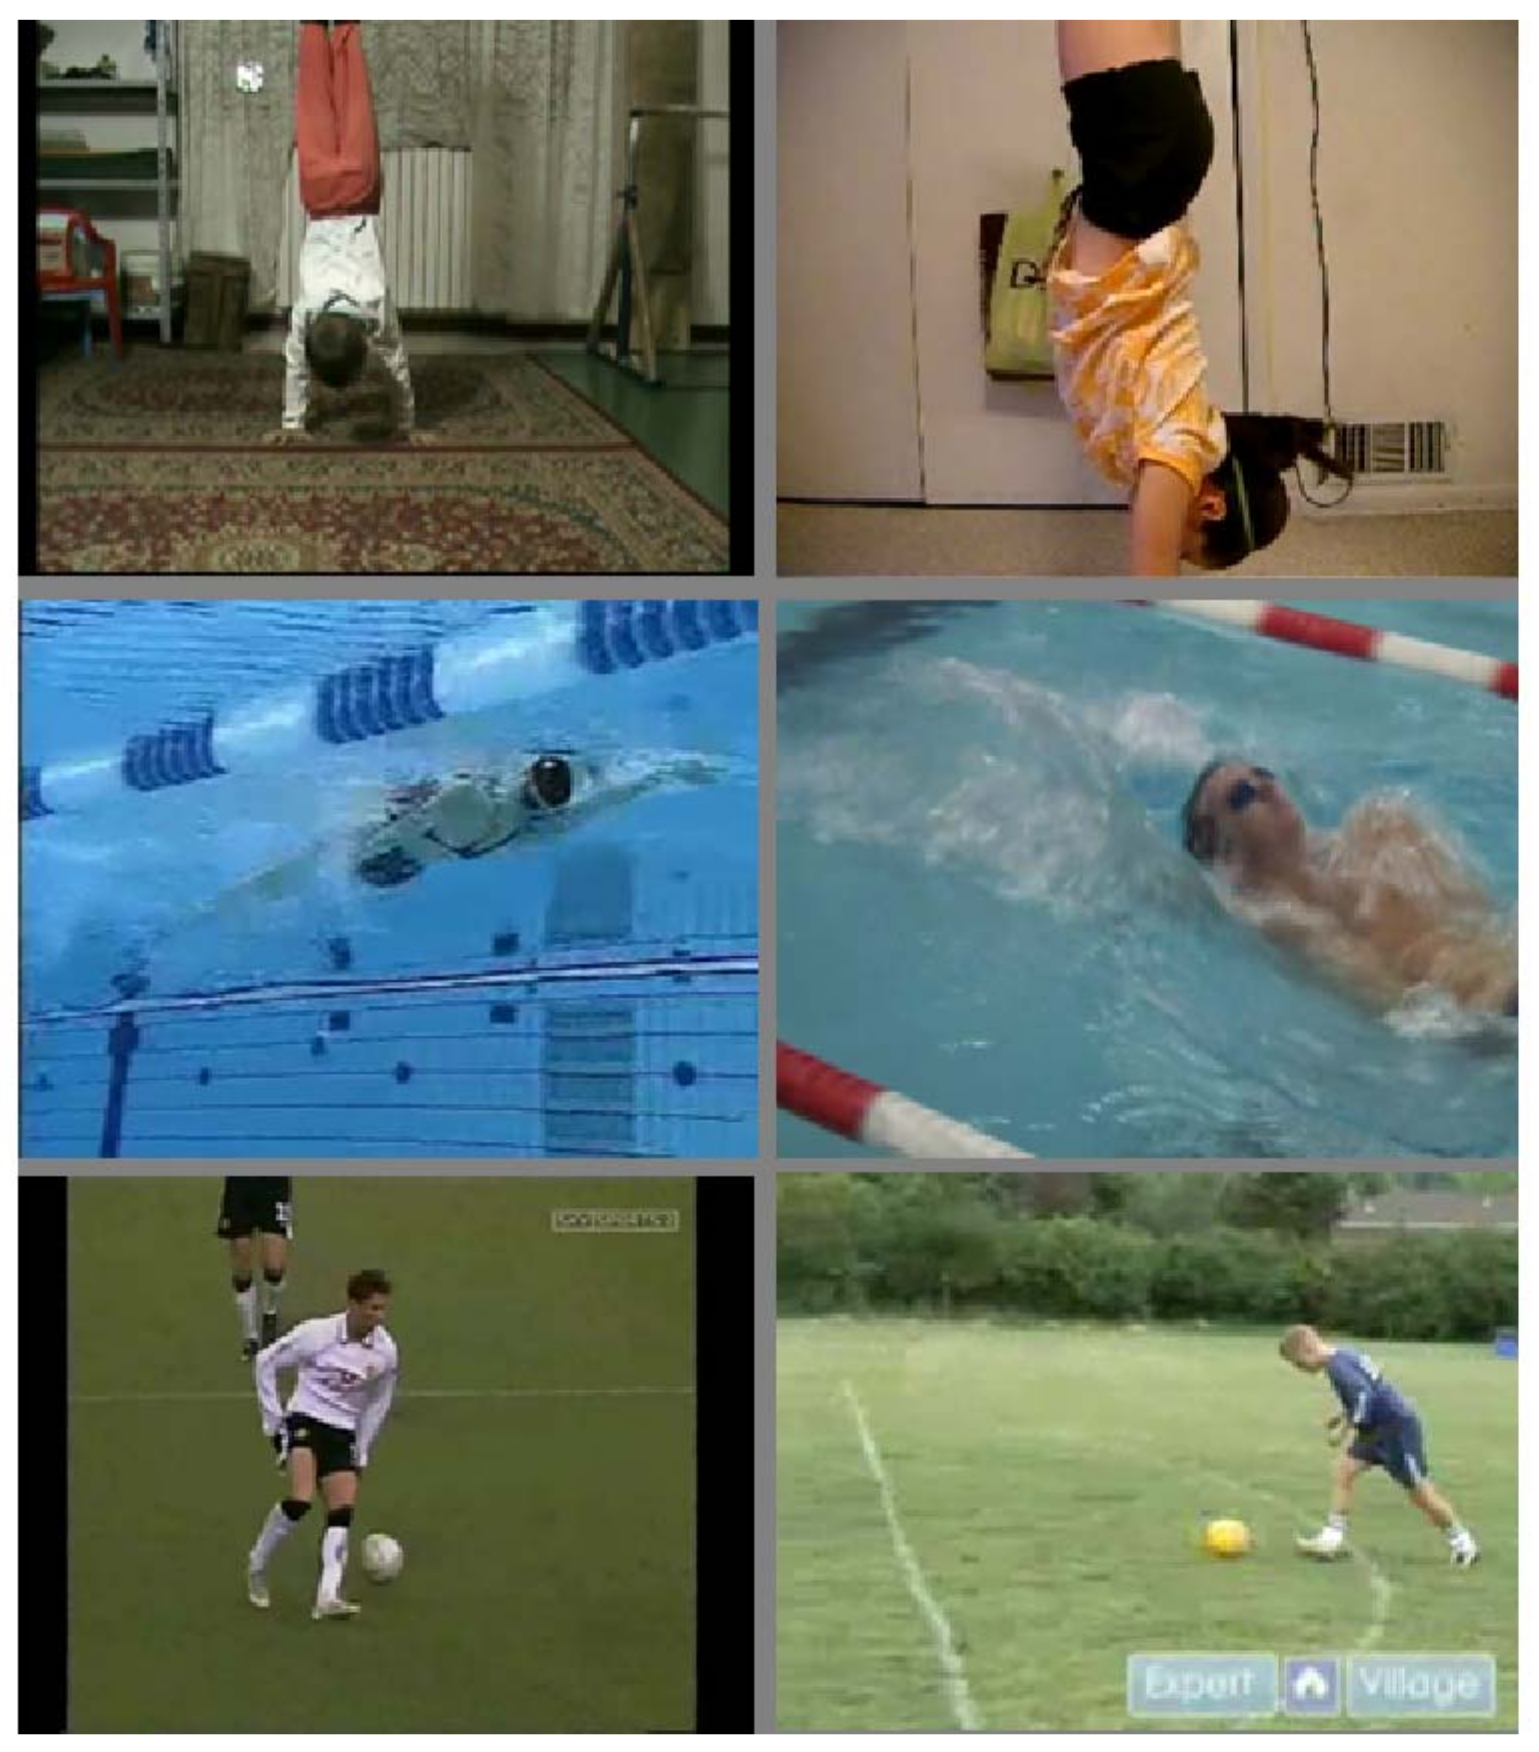
\includegraphics[width=\textwidth]{img_datasets/aslan_same}
        \caption{Example frames of video pairs labeled \textit{same} \cite{kliper-gross_action_2012}}
        \label{fig:aslan_same}
    \end{figure}
\end{minipage}
\hfill
\begin{minipage}[t]{0.4\textwidth}
    \begin{figure}[H]
        \centering
        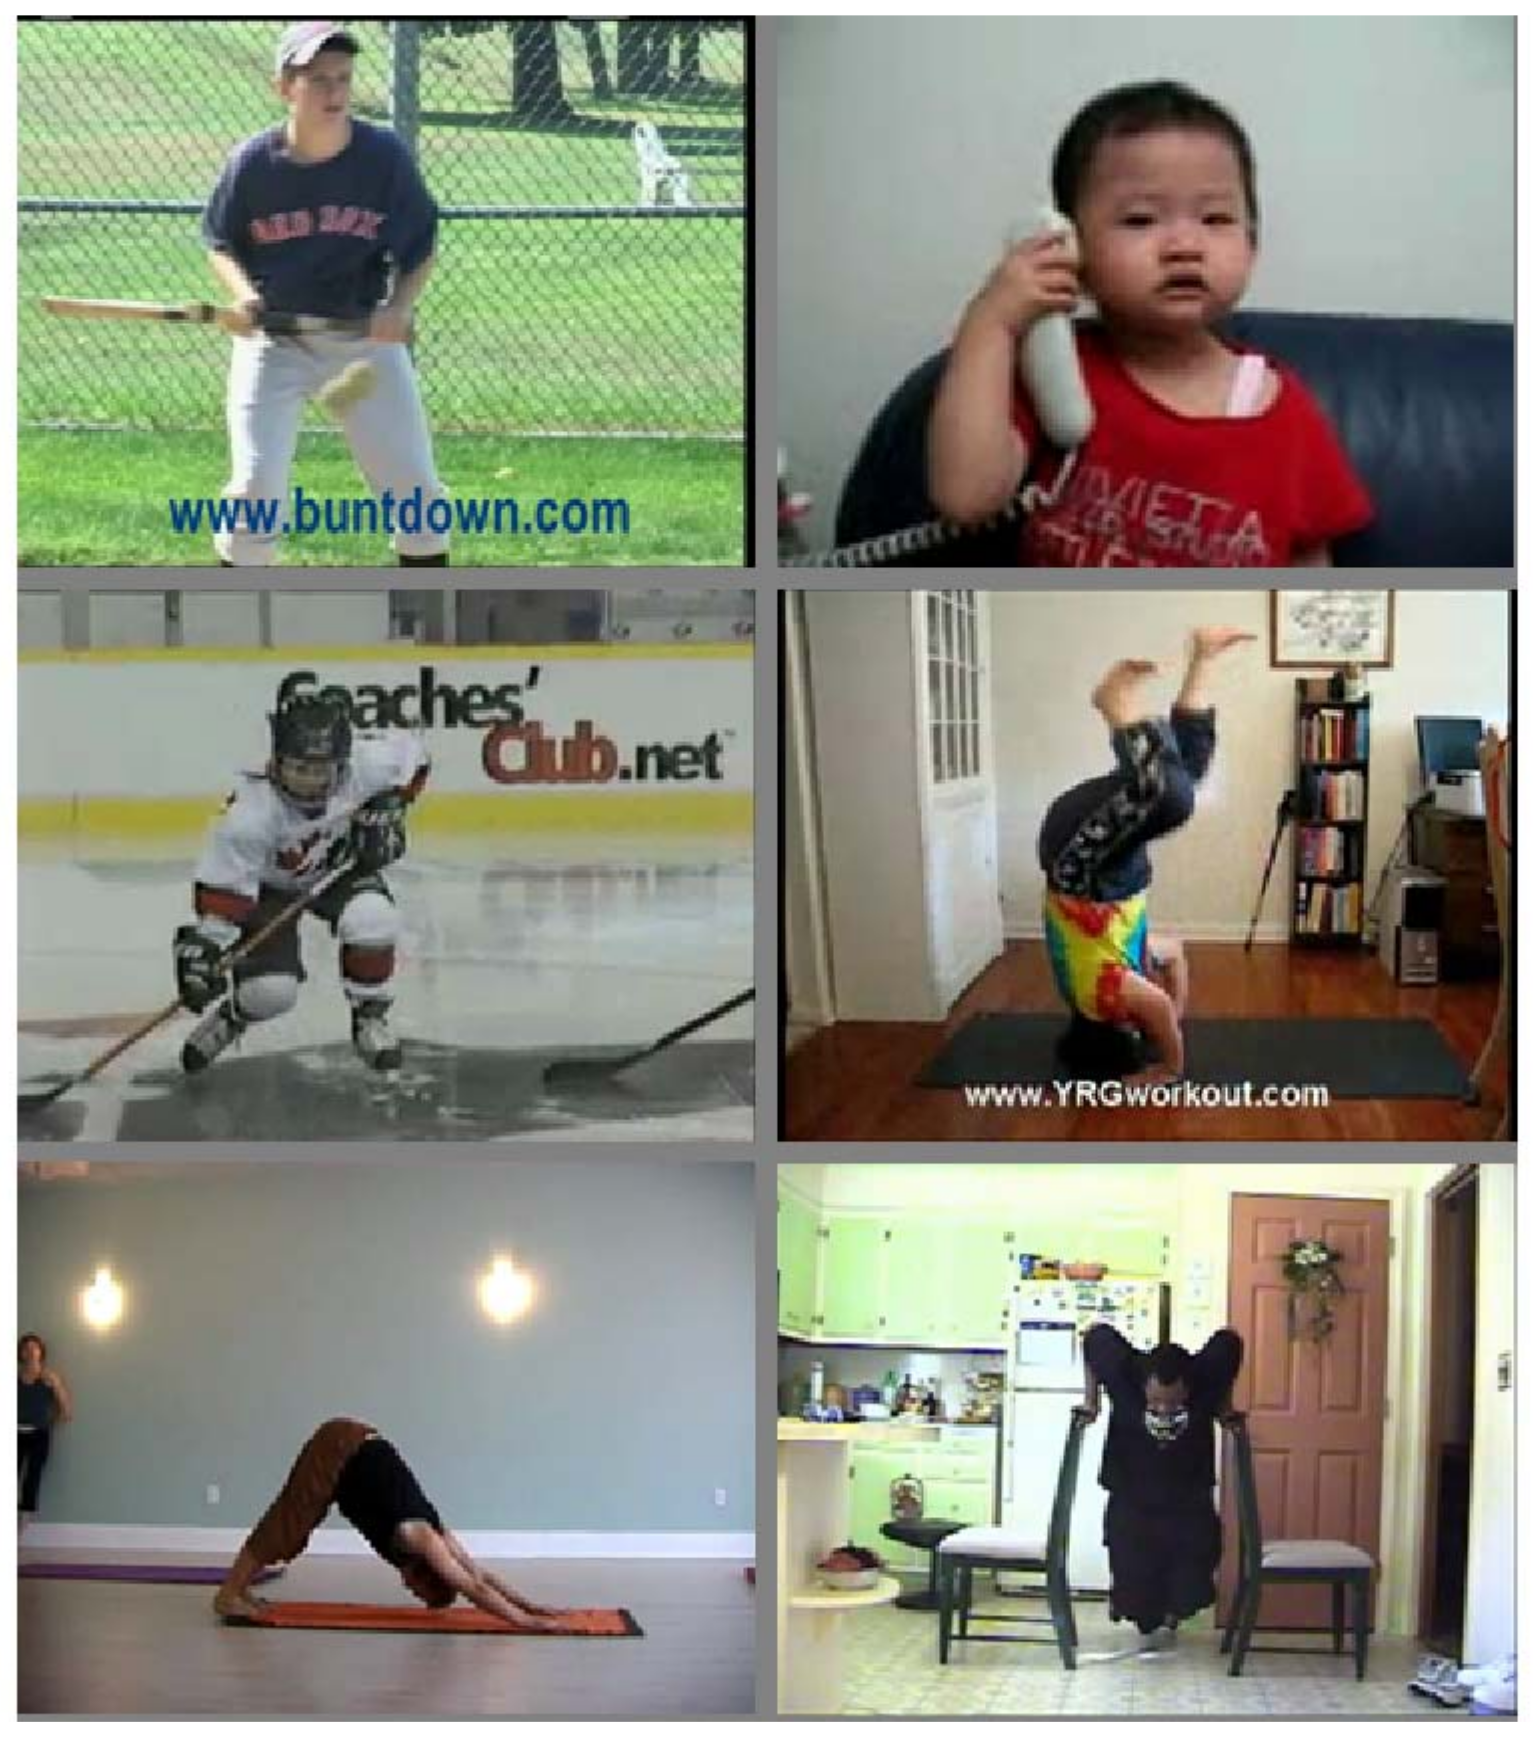
\includegraphics[width=\textwidth]{img_datasets/aslan_different}
        \caption{Example frames of video pairs labeled \textit{not same} \cite{kliper-gross_action_2012}}
        \label{fig:aslan_different}
    \end{figure}
\end{minipage}


\subsubsection{Sports-1M -- 2014}
%\cite{karpathy_large-scale_2014}
The Sports-1M dataset \cite{karpathy_large-scale_2014} was released in 2014 by the Computer Science Department at Stanford University.
The dataset contains links to $1,133,158$ sports videos from YouTube, which have been labeled automatically into $487$ different sports classes by analyzing the text meta-data provided with the videos.

The $487$ action classes are arranged according to a manually created taxonomy with more general classes at the top and more specific classes towards the leaves.
Each class contains about $1000$ to $3000$ videos and about 5\% of the videos have multiple class labels.
The videos are therefore weakly annotated with potentially wrong labels and may provide a lot of variations on the frame level, i.e.\ the actions are not temporally localized in the videos and may be accompanied by unrelated content (e.g. spectators, interviews or scoreboards).

For evaluation, the authors provide a split by assigning 70\% of the videos to a training set, 20\% to a test set and 10\% to a validation set.
Unfortunately around 7\% of the dataset is not available anymore, because the videos were removed from YouTube \cite{ng_beyond_2015}.

Because of the above stated properties of the Sports-1M it is said to be used with caution \cite{kang_review_2016}, although it is the biggest action recognition dataset available to date.

%\subsubsection{THUMOS}
%THUMOS is a large scale dataset (Feichtenhofer)
%
%``Another large scale dataset is the THUMOS dataset [8] that has over 45M frames. Though, only a small fraction of these actually contain the labelled action and thus are useful for supervised feature learning.'' Feichtenhofer 2016


\subsection{Activities of Daily Living (ADL) Datasets}

go on here ??

\subsubsection{URADL -- 2009}
The University of Rochester Activities of Daily Living Dataset (URADL) \cite{messing_activity_2009} was released in 2009.
It contains high-resolution videos of daily-living actions, which were recorded in front of a static background (kitchen) by a tripod-mounted, static camera.

The dataset contains $10$ action classes: answering a phone, dialing a phone, looking up a phone number in a telephone directory, writing a phone number on a whiteboard, drinking a glass of water, eating snack chips, peeling a banana, eating a banana, chopping a banana, and eating food with silverware.
Each action was performed three times by five different actors, resulting in a total of $150$ videos in the datset and $15$ actions per class.

Each video provides a resolution of $1280 \times 720$ pixels at $30$\textit{fps}.
A video contains a complete action and lasts between $10$ and $60$ seconds until the action is finished.

Example frames for the ten action classes are shown in figure \ref{fig:uradl_example}.
\begin{figure}[H]
    \centering
    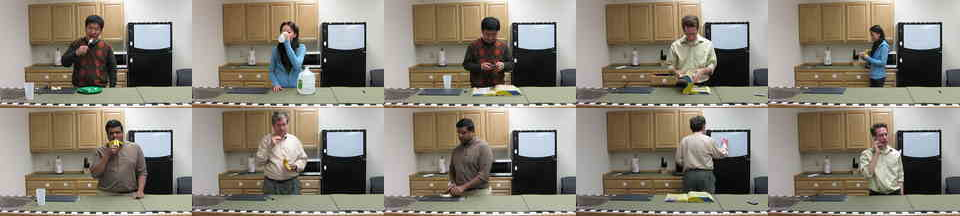
\includegraphics[width=\textwidth]{img_datasets/uradl_example}
    \caption{Example frames for the action classes in the URADL dataset \cite{_university_????}}
    \label{fig:uradl_example}
\end{figure}


%\subsubsection{TUM Kitchen Dataset} \cite{tenorth_tum_2009}


\subsubsection{Multiple Cameras Fall Dataset -- 2010}
\cite{auvinet_multiple_2010}
The Multiple Cameras Fall Dataset was released in 2010 by the University of Montreal, Canada \cite{auvinet_multiple_2010} and contains videos of simulated falls and daily activities recorded with a multi-camera system.
It is designed for developing healthcare vision systems to detect falls of elderly people at home.

The dataset is small and contains the recordings of $24$ events in eight different perspectives, performed by a single actor.
$22$ of the events include a falls, which are performed during confounding actions such as walking, housekeeping and activities with similiar appearance as falls (e.g.\ sitting down or crouching).
$2$ of the recorded events only include confounding actions and no falls.
The scenes include occlusions from furniture or other moving objects (see figure \ref{fig:multiplecamerasfall_example}).
The dataset only provides the raw recordings without action annotations.

\begin{figure}[H]
    \centering
    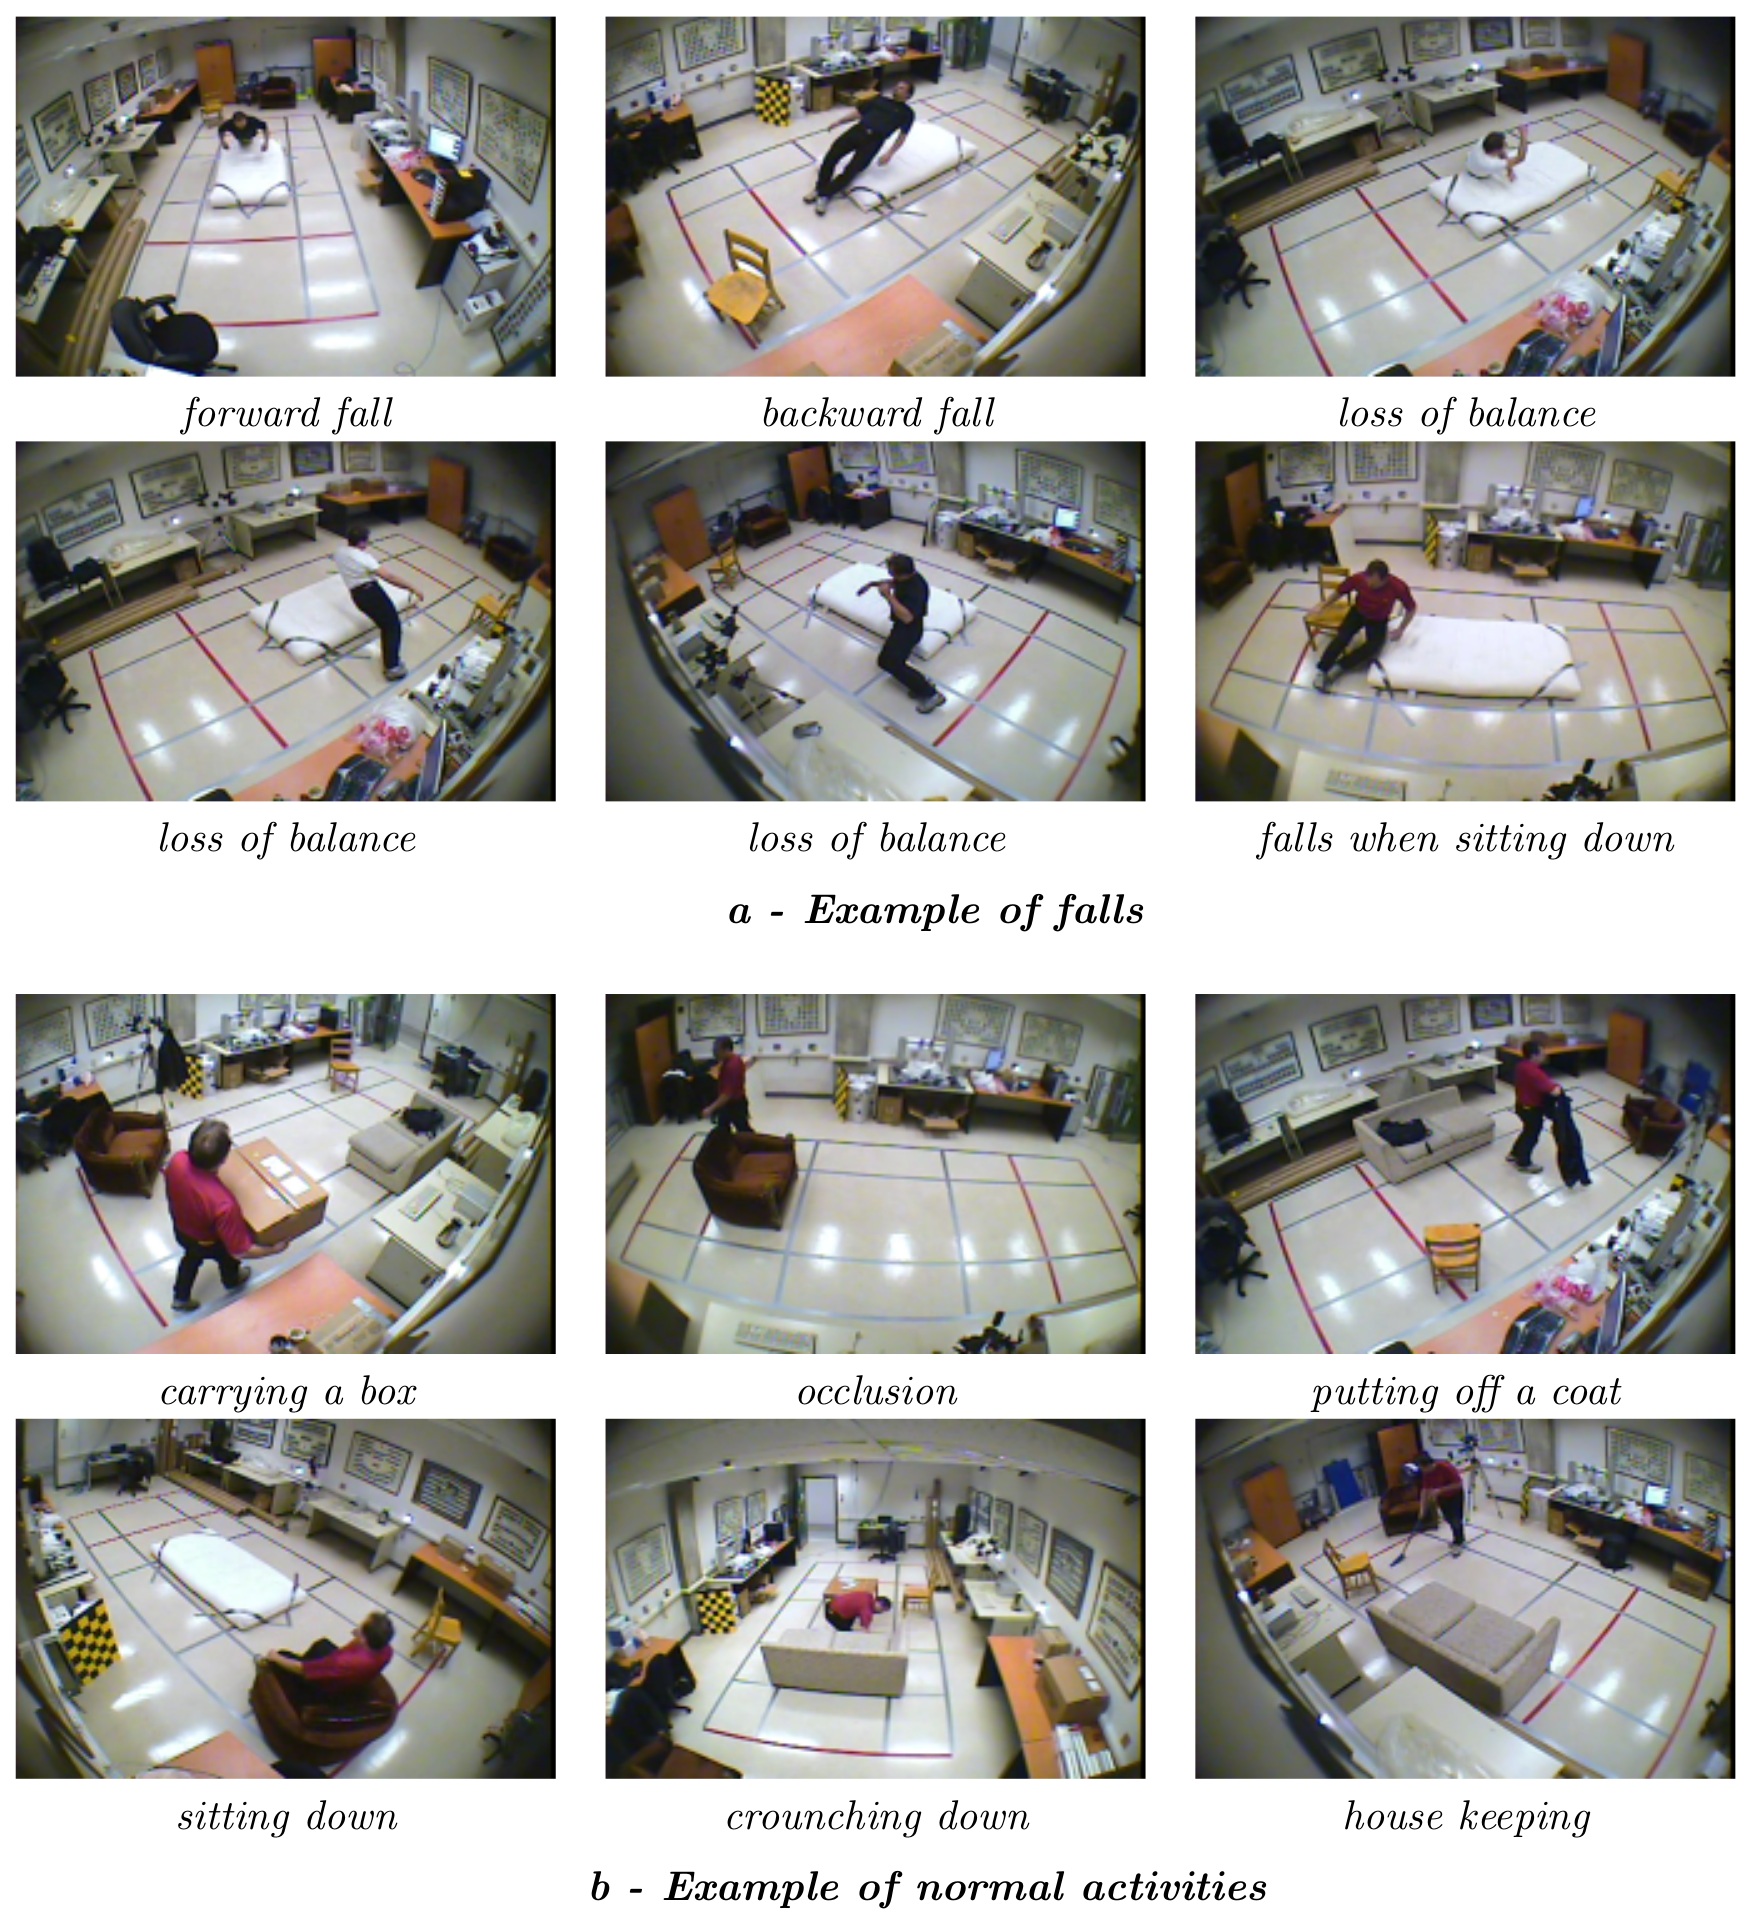
\includegraphics[width=\textwidth]{img_datasets/multiplecamerasfall_example}
    \caption{Example frames of falls (a) and confounding activities performed before or after a fall (b) \cite{auvinet_multiple_2010}}
    \label{fig:multiplecamerasfall_example}
\end{figure}


\subsubsection{MPII Cooking Activities Dataset -- 2012}
\cite{rohrbach_database_2012}
The MPII Cooking Activities Dataset was released in 2012 by the Max Planck Institute of Informatics (Germany) to provide a dataset for fine-grained activity recognition
The dataset contains videos of 12 participant preparing one to six out of $14$ dishes.
The preparation of a dish has been recorded continuously, to apply detection as well as recognition algorithms to the dataset.
In total $44$ videos were recorded with a combined length of $8$ hours featuring $65$ different cooking action classes in $5,609$ annotated action clips.
The videos have a resolution of $1624 \times 1224$ and were recorded in a realistic setting with a stationary camera mounted to the ceiling.

\begin{figure}[H]
    \centering
    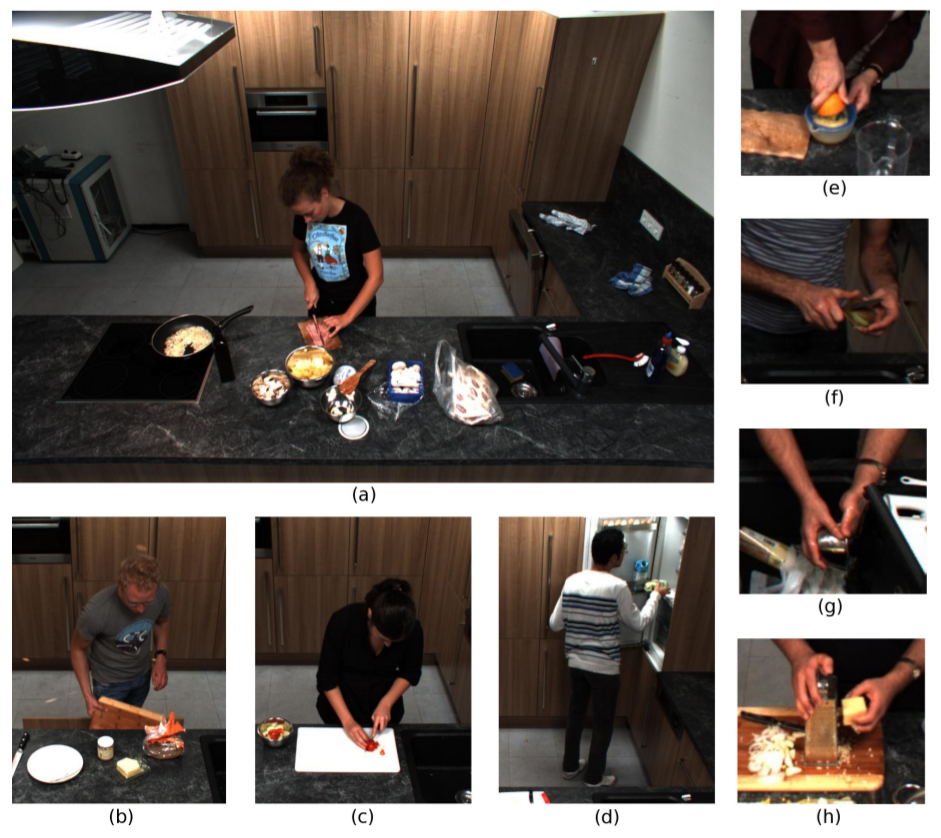
\includegraphics[width=\textwidth]{img_datasets/mpiicooking_example}
    \caption{Example frame and crops of cooking activities. (a)cut slices, (b)take out from drawer, (c)cut dice, (d)take out from fridge, (e)squeeze, (f)peel, (g)wash object, (h)grate. \cite{rohrbach_database_2012}}
    \label{fig:mpiicooking_example}
\end{figure}


%\subsubsection{First Person Activities of Daily Living -- 2012}


\subsubsection{ActivityNet}
\cite{caba_heilbron_activitynet:_2015}
ActivityNet is a large-scale activity recognition dataset released in 2015 by researchers of the Universidad del Norte in Colombia and the King Abdullah University of Science and Technology in Saudi Arabia.
The dataset contains a wide range of videos with daily living activities, which were obtained from YouTube.
The latest release of the dataset (release 1.3 of march 2016, as available from the official website \cite{_activity_????}) consists of annotated links to YouTube videos, organized in $200$ activity classs.
The labels are provided in JSON-format and contain the video-ID, the activity labels along with beginning- and end-time, total video-duration, resolution and url.
A single video can contain multiple activity instances of different activity classes.
The majority of videos is available in a resolution of $1280 \times 720$ pixels and lasts between $5$ and $10$ minutes.

The database is divided as follows:
\begin{itemize}
    \item $10,024$ training videos (containing $15,410$ activity instances) 
    \item $4,926$ validation videos (containing $7,654$ activity instances)
    \item $5,044$ testing videos (labels withheld) 
\end{itemize}

Besides providing annotated video-links, a taxonomy of the daily living activities in the ActivityNet hierarchy with four levels of granularity.
The top-level categories being:
\begin{itemize}
    \item Personal Care
    \item Eating and Drinking
    \item Household
    \item Caring and Helping
    \item Working
    \item Socializing and Leisure
    \item Sports and Exercises
\end{itemize}

Following figure \ref{fig:activitynet_taxonomy} shows the visualization of the activity category \textit{Household}.
\begin{figure}[H]
    \centering
    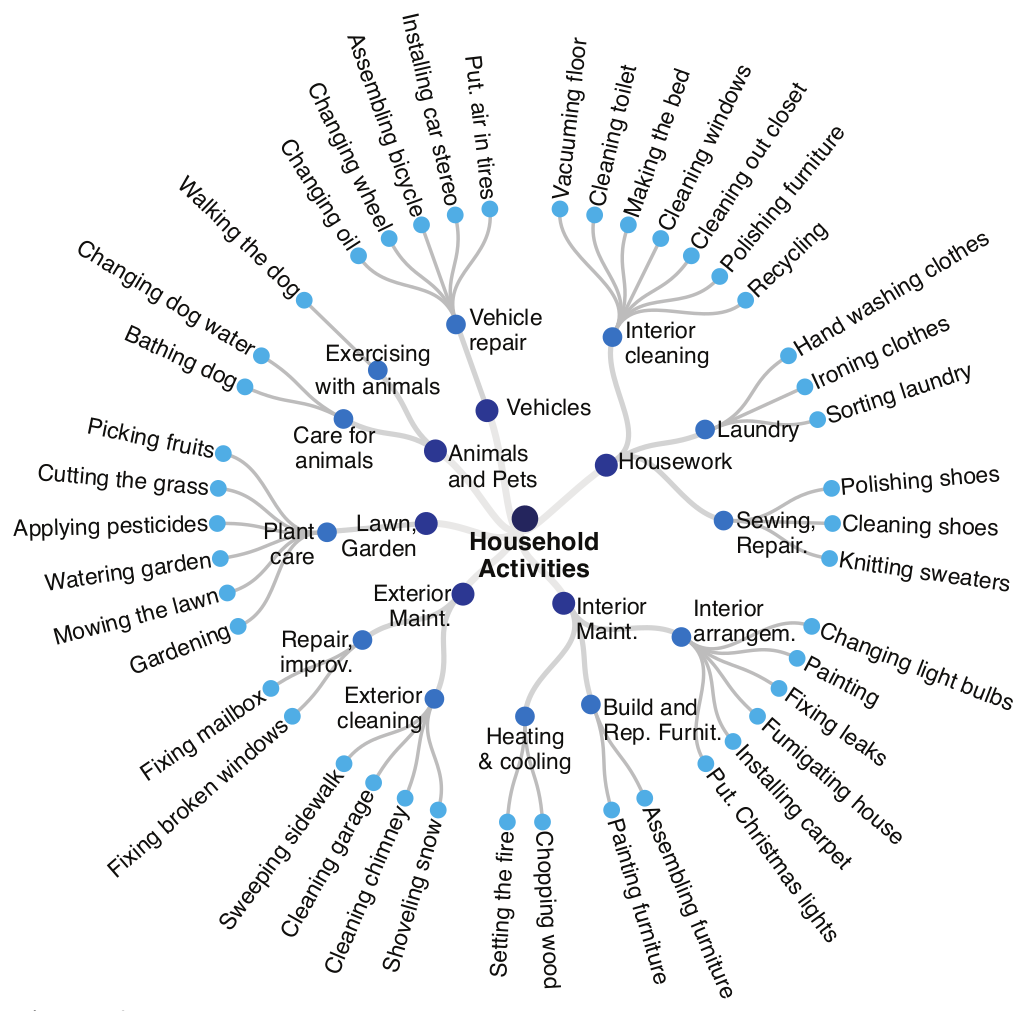
\includegraphics[width=0.7\textwidth]{img_datasets/activitynet_taxonomy}
    \caption{Taxonomy of top-level activity category \textit{Household}}
    \label{fig:activitynet_taxonomy}
\end{figure}

ActivityNet is the biggest manually annotated video-dataset available to date.
It is applicable for detection as well as recognition algorithms and was used in the ActivityNet Challenge along CVPR 2016.
Although not explicitly mentioned by the authors, it is unclear how many of the videos are currently still available on YouTube (see Sports-1M).

\subsection{Algorithm Testing Protocol}

The creators of UCF-101 and HMDB-51 provide three splits of their datasets into training- and testing-data.
The standard evaluation procedure is to report the average accuracy over those three splits, which the authors follow in this work as well.
simonyan zisserman two-stream approach

``In [4], Gao et al. presented a comprehensive study on the influence of the evaluation protocol on the final results. It was shown that the use of different experimental configurations can lead to performance differences up to 9\%.''
``Action recognition methods are usually directly compared although they use different testing protocols or/and datasets (KTH1 or KTH2), which distorts the conclusions.''
cite sequential deep learning for human action recognition.
